\documentclass[16pt,a5paper,oneside]{book}
\usepackage[T2A,T1]{fontenc}
\usepackage[utf8]{inputenc}
\usepackage[english,russian]{babel}
\usepackage[margin=1cm]{geometry}
\usepackage{wrapfig}
\usepackage{graphicx}
\graphicspath{{/home/valentin/PhpstormProjects/Master100pages/src/images/}}

\begin{document}

\title{ИСТОРИЯ ГРУППЫ «МАСТЕР»}
\author{Владимир Марочкин}
\date{2003}

\begin{figure}
    \centering
    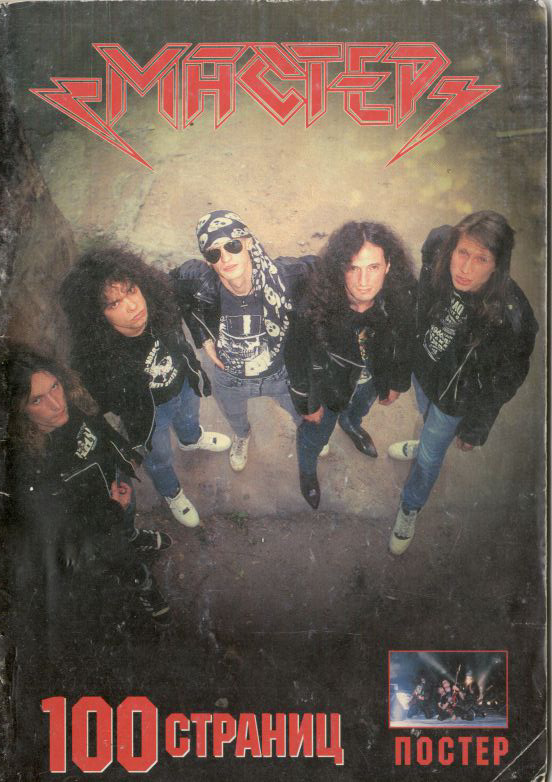
\includegraphics[scale=0.6]{Cover1}
\end{figure}

\begin{figure}
    \centering
    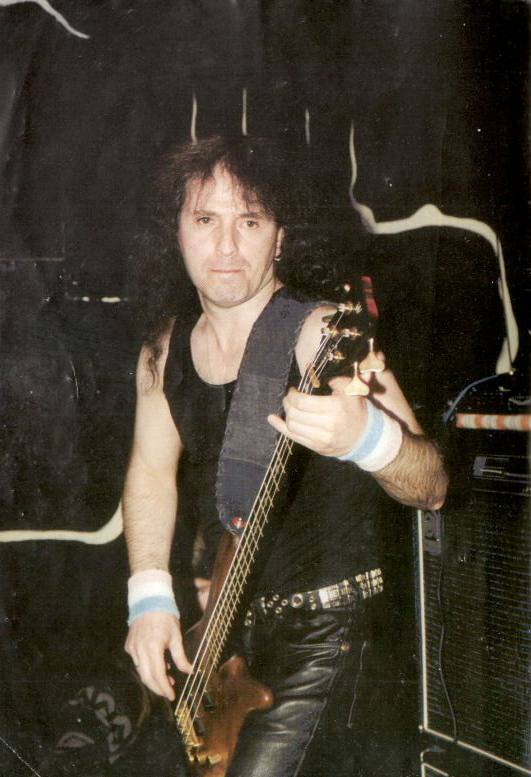
\includegraphics[scale=0.6]{Cover2}
\end{figure}

\maketitle

Рок-энциклопедии датируют рождение группы «Мастер» осенью 1986 года, когда четверо музыкантов группы «Ария» — Алик
Грановский, Андрей Большаков, Кирилл Покровский и Игорь Молчанов — объявили руководителю ансамбля Виктору Векштейну,
что покидают его группу и создают свою собственную. На самом деле, как и положено, все началось гораздо раньше, 12 лет
назад, а 12 лет, как утверждают астрологи, составляют целый жизненный цикл\ldots
\newline
\newline
Дождливой осенью 1974 года 15-летний Алик Грановский проводил свои свободные вечера (а свободными были почти все вечера)
дома у гитариста Сергея Потемкина, вместе с которым они пытались создать рок-группу. Однако совместное музицирование,
как правило, заканчивалось достаточно прозаически. Потемкин поиграет на гитаре, потом подойдет к колонкам, сеточку
потрогает и скажет грустно и мечтательно: «Да, нужна аппаратура! Нужно много аппаратуры\ldots». Да где же ее взять-то
было в 1974 году?! Так и не удалось тогда создать группу, хотя впоследствии поиграли вместе Алик и Сергей в нескольких
составах, в том числе и профессиональных. А дружба эта юношеская в дальнейшем существенно повлияла на биографию группы
«Мастер». Сергей Потемкин, разглядев в юном Грановском талантливого музыканта, на длительное время сделался его
ангелом-хранителем, направляя путь своего друга в нужном направлении, сводя с нужными людьми и подыскивая необходимых
музыкантов даже ценой развала собственных проектов.

Андрей Большаков — другой лидер «Мастера» — в 1974 году поступил в Московский полиграфический институт. Одновременно он
играл группе «Шестое чувство», которая была создана еще во время учебы в московской средней школе № 185. Группа, как
тогда было принято, исполняла на танцах «фирменный» репертуар из произведений звезд английской рок-сцены — групп
«Т.Rex», «Creedence» и «Slade».

\begin{figure}
    \centering
    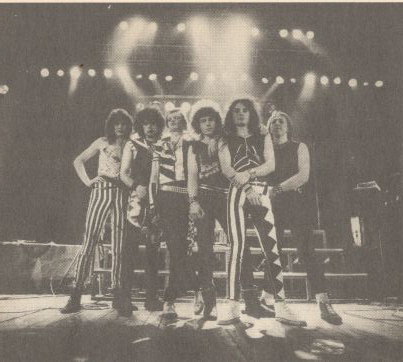
\includegraphics[scale=0.9]{Image01}
    \caption{\textit{
        Первый состав группы «Мастер» (слева-направо): Игорь Молчанов, Кирилл Покровский, Андрей Большаков, Сергей
        Попов, Алик Грановский и Александр Арзамасков. Май 1987 год.
    }}
\end{figure}

Девятиклассник Александр Елин, будущий автор текстов бессмертных хитов «Воля и Разум», «Встань, страх преодолей»,
«Здесь куют металл», в 1974 году впервые попал на пластиночную «толкучку». Первой его добычей стал альбом «Survival»
группы «Grand Funk Railroad», что на всю жизнь предопределило тягу Елина к «тяжелому» року.

Будущий звукорежиссер группы «Мастер» Андрей Лебедев по прозвищу «Крустер» в 1974 году был принят в группу «Млечный
путь», в которой в то время играли студенты МИЭМ Александр «Билл» Мирошников (клавиши), Сергей «Шеф» Попов (гитара,
вокал), Павел Бабердин (бас, вокал) и будущий лидер группы «ДК» Сергей Жариков (барабаны). Андрея в группу привел Билл,
который тогда ухаживал за его сестрой. Едва началась настоящая, «живая» музыка, Крустер «забил» на учебу в ПТУ и все
время стал проводить со своими старшими друзьями — даже ходил с ними в институт, фактически прослушав институтский курс
лекций по прикладной математике. Ему «сделали» студенческий билет, который Андрей показывал на институтской проходной,
а на занятиях его представили как нового студента, и все прошло. Крустеру же велели сидеть на лекциях с умным видом, что
он и делал: сидел, волос у виска на палец накручивая, и терпеливо ждал, когда можно будет наконец пойти
репетировать\ldots

\begin{wrapfigure}{L}{0.5\textwidth}
    \centering
    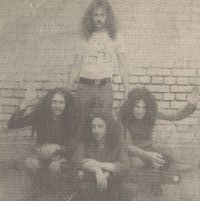
\includegraphics[scale=0.8]{Image02}
    \caption{\textit{
        Первая группа Грановского. Алик на этом снимке сидит справа, а рядом с ним - Сергей Потемкин и Юрий Камышников
    }}
\end{wrapfigure}

В мировой рок-музыке 1974 год также являлся весьма примечательным. Будущий всемирный кризис «хард-рока» как массового
музыкального жанра еще никак себя не проявлял, и 1974 год скорее можно было назвать временем расцвета «тяжелой музыки»,
хотя все глобальные открытия жанра уже состоялись\ldots

Американская группа «Grand Funk» записала пластинку «Shinin' On», и песня «Locomotion» с этой пластинки возглавила
хит-парад США.

Британская группа «Slade» вошла в 1974 год с песней «Merry Xmas Everybody», поднявшейся до 1 места в национальном
хит-параде, а уже в феврале закрепила свой успех попаданием логнплея «Old, News, Borrowed \& Blue» на первое место в
списке лучших альбомов Соединенного Королевства.

\begin{wrapfigure}{R}{0.5\textwidth}
    \centering
    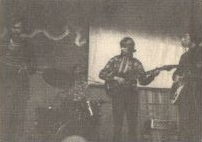
\includegraphics[scale=0.8]{Image03}
    \caption{\textit{Группа «Шестое чувство»}}
\end{wrapfigure}

Группа «Deep Purple» выпустила сразу два альбома — «Burn» и «Storm-bringer», а голос Дэвида Ковердейла, звучащий на этих
пластинках, стал путеводной нитью для многих советских групп тяжелого направления.

\begin{figure}
    \centering
    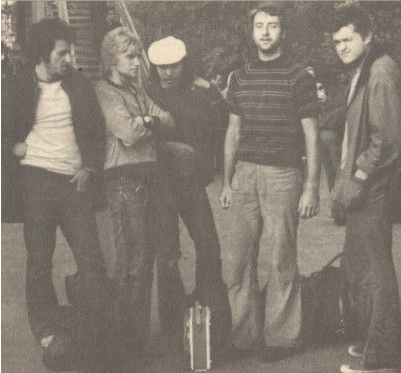
\includegraphics[scale=0.9]{Image04}
    \caption{\textit{
        «Млечный путь» (слева направо): звукооператор Евгений Морозов, Павел Бабердин, Андрей «Крустер» Лебедев,
        Александр Мирошников и Сергей Жариков
    }}
\end{figure}

Группа «Rush» записала в 1974 году дебютный альбом и отправилась в турне для его раскрутки.

В 1974 году группа «King Crimson» выпустила альбом «Red», после чего Роберт Фрипп распустил группу.

«Это — мой самый любимый альбом, — говорит Алик Грановский, — он до сих пор цепляет какие-то мои внутренние струнки».

«А моим самым любимым альбомом тогда был «Larks Tongues In Aspic» (более ранний «King Crimson»), — вспоминает Андрей
Большаков. — Я всегда любил необычное, я не любил «квадратное». Хотя парадокс в том, что любил я одну музыку, а
играли-то мы совсем другое, например, «Slade», — куда уж примитивнее и проще: два аккорда! Или «T. Rex»: три аккорда в
лучшем случае\ldots»

В 1975 году пути Грановского и Большакова едва не пересеклись: они оба побывали на сейшене группы «Второе Дыхание»,
проходившем в физкультурном зале физико-математической школы N279, что расположилась неподалеку от ВДНХ, напротив
кинотеатра «Космос». Зал был полон хиппи. На полу лежали физкультурные — на них валялся народ: кто-то курил, кто-то
пытался заниматься любовью. Люди висели даже на шведских стенках, а на сцене рубилась группа «Второе Дыхание»,
исполнявшая пьесы из репертуара «Сreаm», Джими Хендрикса (Jimi Hendrix) и Билли Кобхома (Billy Cobham). Но Грановский и
Большаков не заметили друг друга, может быть даже безразлично прошли мимо, лишь скользнув взглядом, а может, они и вовсе
были в разных концах битком набитого зала, а потому и не видели друг друга, — это неважно, главное, что они оба там были
и могли познакомиться. Но этого не произошло, видимо, создавать совместную группу было еще рано. Бывают такие странные
дни, когда люди встречаются, но нечто не дает их биографиям пересечься\ldots

В 1976 году Большаков вместе с приятелем из своей старой группы перебрался в ансамбль «Фламинго», состоявший из
венгерских студентов, обучавшихся в МГУ. Это был серьезный шаг вперед, потому что группа «Фламинго» регулярно выступала
на студенческих сейшенах в различных московских вузах, а кроме того пыталась играть достаточно сложную музыку, в ее
репертуаре была даже одна пьеса из репертуара «Emerson, Lake \& Palmer», правда, скорее популярная, чем сложная\ldots

\ldotsВ том же 1976 году Сергей Потемкин через своего друга Мишу Павлова познакомил Грановского с музыкантами группы
«Млечный Путь». К этому времени музыканты первоначального состава уже закончили свой вуз и были распределены в различные
нии и КБ, и работа поглотила их. Теперь Млечный Путь выступал в составе. Андрей Крустер (гитара, вокал), Павел Бабердин
(гитара, вокал). Алик Грановский (бас), Сергей Потемкин (гитара), Сергей «Шелл» Шелудченко (барабаны). Сергей Жариков
продолжал сочинять песни для группы, он тогда написал целый и жутких, леденя кровь текстов, например «Голодная чума» или
«Лучше смерти будет только смерть». Но вскоре «накрылась» репетиционная база «Млечного Пути» в ДК «Сетунь», в итоге
группа распалась, и Грановский остался вдвоем с Крустером. Они еще когда познакомились, почувствовали себя братьями по
духу, ведь им было по 18 лет и они оба любили выкручивать ручку громкости до отказа, чтобы было очень громко, очень
конкретно и очень жестоко.

\begin{figure}
    \centering
    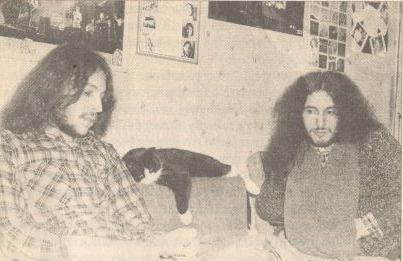
\includegraphics[scale=0.8]{Image05}
    \caption{\textit{Андрей Крустер и Алик Грановский. Первая фотосессия будущих звезд прошла прямо на флэту}}
\end{figure}

Андрей и Алик сразу решили, что создадут новую группу, но так как репетировать было негде, они просто напевали песни,
стуча по коленкам. Крустер пел за гитару и как бы играл на барабанах, а Грановский изображал бас и тоже играл на
барабанах. Они репетировали каждую свободную минуту — и на работе, и дома. Исподволь шло дальнейшее сближение
характеров: за два года подобных репетиций они стали понимать друг друга буквально с полуслова и полувзгляда, что очень
сильно пригодилось позже, когда им все-таки удалось собрать свой ансамбль. Говорят, что так слаженно, как играли вместе
Грановский и Крустер, тогда не играл никто\ldots

В 1977 году Большаков играл в группе «Фаворит», исполнявшей исключительно произведения Элиса Купера (Alice Cooper). Там
пел Валерий Третьяков, начавший свою музыкальную биографию еще в 1966 году, в группе «Авангард», на гитаре играл
Александр Иншаков, на бас-гитаре Владимир Черепанов, а за барабанами работал бывший музыкант ВИА «Веселые Ребята», чье
имя историей утеряно. «Фаворит» полгода репетировал, но выступил лишь один раз, в какой-то школе на юго-западе столицы.
Вскоре после этого Валер Черепанов устроился на работу звукорежиссером в Театр Имени Ленинского комсомола и покинул
группу. Замену ему так и не нашли, и в результате группа распалась\ldots

Удивительно, но к 1977 году развалилось большинство тяжелых команд, задавших тон в музыке первой половине 70-х.
Ритчи Блэкмор (Ritchie Blackmore) ушел из «Deep Purple», следом за ним группу оставил Дэвид Ковердэйл (David Coverdale),
после чего ансамбль распался окончательно. То же и Оззи Осборн (Ozzy Osbourne) покинул «Black Sabbath». Дэвида Байрона
(David Byron) уволили из «Uriah Heep» за беспробудное пьянство. После неудачи очередного альбома прекратила
существование группа «Grand Funk Railroad». Вокалист группы «Led Zeppelin» Роберт Плант (Robert Plant) попал в
автокатастрофу и у группы настала длительная пауза как в концертной, так и в студийной работе. У всех «стариков» по тем
или иным причинам в 1977 году случилась пауза. Кроме того, 16 августа 1977 года в своем доме в Мемфисе умер Кароль
рок-н-роса Элвис Пресли (Elvis Presley)\ldots

В 1978 году Грановский и Крустер предприняли попытку прорваться на профессиональную сцену. Захватив с собой барабанщика
«Млечного Пути» Сергея Шелудченко и соло-гитариста Романа Амиридиса (в будущем — гитарист группы «СВ»), они отправились
на прослушивание в Саратовскую филармонию. Получасовая импровизация произвела сильное впечатление на руководителей
филармонии, но так как у ребят еще не было ни репертуара, ни должного концертного опыта, руководители саратовской
культуры предпочли им другой самодеятельный коллектив — студенческую группу Бари Алибасова «Интеграл». Грановский и его
товарищи вернулись из Саратова в Москву ни с чем, их первый профессиональный блин вышел в соответствии с пословицей —
комом\ldots

Покинув «Фаворит», Большаков не играл почти два года. Он тогда познакомился со своей будущей женой Ладой и все время,
свободное от лекций и сдачи экзаменов, проводил с ней. Даже гитару продал\ldots

Но вот настал 1980 год, печально знаменитый смертями Джона Леннона (John Lennon), барабанщика «Led Zeppelin» Джона
Бонэма (John Bonham), вокалиста «AC/DC» Бона Скотта, французского шансонье Джо Дассена (Joe Dassin) и русского барда
Владимира Высоцкого. Но люди, посвященные и таинственный ход судьбы, сказали бы, что эти смерти — жертвенные, они
готовят приход новой эпохи\ldots

В один осенний вечер 19800 года Александр Иншаков, с которым Большаков играл в «Фаворите», позвонил Андрею и пригласил
его в свою группу «Карусель»\ldots вокалистом. Это удивительно, но Большаков согласился! Андрею только что исполнилось
24 года, а это именно тот возраст, когда люди начинают делать себе имя, карьеру, добиваться конкретного успеха. Какие-то
пробы пера и поиски себя к этому возрасту уже проделаны и человек уже представляет, кем хочет быть. В 1980 году
Большаков как раз окончил полиграфический институт, получил диплом и был распределен на работу в типографию. Однако
Андрей не собирался всю свою жизнь связывать с подобной деятельностью, он хотел быть музыкантом и потому принял первое
же более или менее реальное предложение.

\begin{figure}
    \centering
    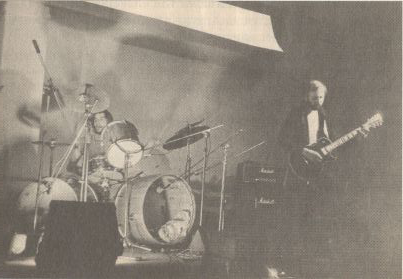
\includegraphics[scale=0.8]{Image06}
    \caption{\textit{«Коктейль»: Шатуновский и Иншаков на концерте}}
\end{figure}

В группе Иншакова, сразу после прихода Большакова переименованной в «Коктейль», также играли Андрей Бутузов (бас-гитара,
ныне «Кроссроудз») и Андрей Шатуновский (барабаны), которого чуть позже сменил Павел Чиняков (экс-«Альянс»). Чуть позже
к группе присоединился вокалист Сергей Перфилов, а Большаков стал вторым гитаристом, хотя по-прежнему пел часть
программы, исполняя песни, созданные им самим. Группа играла актуальную для того времени смесь «хард-рока» и «новой
волны», много выступала и имела довольно устойчивую популярность среди любителей рока, а хит «Спартак — чемпион!» знала,
похоже, вся страна, хотя по радио «Коктейль» не передавали и по телевизору не показывали\ldots

\begin{wrapfigure}{L}{0.5\textwidth}
    \centering
    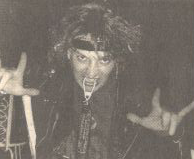
\includegraphics[scale=0.9]{Image07}
    \caption{\textit{Артур Беркут в 1979 году}}
\end{wrapfigure}

Большую часть 1980 года Грановский и Крустер провели в поисках вокалиста. Однажды, кажется, в конце лета, Грановского
занесло на базу группы «Волшебные Сумерки», в которой на гитаре играл Владимир Холстинин, на бас-гитаре — Виталий
Дубинин, а пел Артур Беркут. Грановский прослушал репетицию, после чего подошел к Артуру и позвал его в свою новую
группу: «Ты клево поешь, давай, если хочешь, будешь у нас работать!». Беркут неожиданно согласился: «Да, я хочу, и я
буду у вас вокалистом!». Они договорились созвониться в течение недели, однако примерно в то же время Артура позвали в
«Автограф» и он принял приглашение. «Автограф» являлся официальной группой, что делало повседневную жизнь ее музыканта
стабильной и обеспеченной, в то время как жизнь андеграундной команды представляла собой абсолютную неопределенность,
когда музыканты не только не знали, что будет завтра, но и не ведали, чем закончится сегодняшний концерт: поедут они
после финального крещендо домой или в ближайшее отделение милиции (а оттуда — в тюрьму или в дурдом)?

Артур Беркут еще будет петь в группе Грановского, но произойдет это лишь 16 лет спустя. А пока Грановский и Крустер,
расстроенные отказом Артура, перебирали знакомых вокалистов, отсевая их одного за другим. Кто-то абсолютно не подходил
по музыкальным пристрастиям, кто-то пел слишком похоже на Ковердэйла, но так тогда пели многие, а нашим друзьям хотелось
чего-то необычного. Вдруг раздался звонок в дверь, и в квартиру влетел запыхавшийся Сергей Шутов, известный
андерграундный художник, и с порога сообщил, что накануне он слышал девчонку, которая поет, как Роберт Плант (Robert
Plant). «Девчонка-вокалистка? Да нет, такого не может быть!» — с ходу отверг предложение Алик. «А почему нет?! — не
сдавался Шутов. — Женский вокал это же необычно!» В конце концов, он убедил Грановского и Крустера подняться с дивана и
прослушать необычного кандидата. Звали ее Алеся Троянская. Она взяла гитару, спела несколько песен из репертуара «Led
Zeppelin», и ее голос настолько очаровал компаньонов, что Грановский и Крустер предложили Троянской сотрудничество.

Новой группе дали имя «Смещение». Название придумал Грановский, вернее, не придумал, а вспомнил: так называлась первая
школьная группа, в которой он играл. Первый концерт «Смещения» прошел в конце осени 1980 года в трамвайном депо на
Таганке. Народ был просто ошарашен — такого в Москве еще не видели и не слышали. «Тогда все играли хард-рок без
каких-либо вариаций, а мы не хотели играть, как все, поэтому нашей музыке было присуще смещение, — вспоминает
Грановский. — Мы играли не только «тяжело», но и вели поиск в прогрессивном жанре. Мы не ограничивались рамками просто
песни, в нашей музыке было очень много импровизации». Не менее серьезным было отношение к внешнему виду и шоу. Они не
топтались на одном месте, как тогда было принято, а неустанно двигались по сцене. Одетая в желтый комбинезон Алеся то
носилась по сцене, то садилась на шпагат, то извлекала из ниоткуда огромный надувной молоток и лупила им по головам
ближних зрителей. Андрей прозвал ее «Трактор Беларусь», потому что голос у нее был луженый, она не столько пела, сколько
орала, у нее не существовало тональностей, вернее была одна собственная тональность, в которую музыканты почему-то
попадали. Троянская пела про «голодную чуму», про «вторую первую любовь», про «дорогу в рай», про то, что «лучше смерти
будет только смерть», а также другие страшные и веселые песни.

\begin{wrapfigure}{L}{0.5\textwidth}
    \centering
    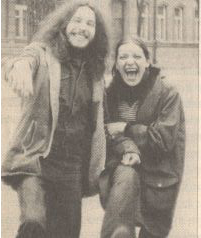
\includegraphics[scale=0.9]{Image08}
    \caption{\textit{«Смещение»: Крустер и Алеся Троянская}}
\end{wrapfigure}

Группа «Смещение» просуществовала недолго, всего полтора года, сыграв за это время лишь десять концертов. Но вся эта
прелюдия, все события, происходившие тогда с музыкантами, были необходимы для будущего «выстрела». Записей «Смещения» не
осталось, но один из хитов — «Таран» — впоследствии будет записан, и в виде бонуса выйдет на альбоме «Лабиринт» группы
«Мастер».

Группы «Коктейль» и «Смещение» были весьма популярны, их выступления проходили при полном зале, несмотря на то, что
рок-концерты в те времена могли принести неприятности и музыкантам, и зрителям. Эти концерты не являлись официальными —
с флайерами, афишами и объявлениями в газетах, как это принято сейчас. Это был настоящий андеграунд (русский аналог
этого слова — подполье). Концерты «заряжались» по телефону: подпольные менеджеры звонили музыкантам и предлагали
выступить, и музыканты чаще всего соглашались. Билеты также распространялись по телефону: устроители концерта
обзванивали знакомых и сообщали, что приблизительно тогда-то состоится концерт, все нормально, сидите на телефоне и
ждите, а когда будут «тикета» (от англ. ticket — билет), мы перезвоним. Место для встречи зрителей тоже выбиралось из
соображений конспирации, как правило, «стрелка» (так на рокерском слэнге обозначалось место и время встречи) назначалась
в метро, за остановку до нужной станции. Когда собиралась вся запланированная публика, руководитель давал команду
грузиться в подошедший поезд и вез всех к месту концерта.

Билетами служили, как правило, разрезанные пополам открытки с каким-нибудь необычным штампом. Например, на билетах у
«Смещения» стоял штамп «Диспансеризация», который их директор Артур Гильдебрандт умыкнул в какой-то поликлинике. «И мы
никогда не распределяли деньги там, где отыграли, — вспоминает Алик Грановский. – Это было очень опасно. Как правило, мы
встречались в метро, скажем, на «Колхозной», в центре зала, и распределяли зарплату\ldots» Такая конспирация, к
сожалению, была необходима, потому что попасться с «деньгой на кармане» во время концерта обозначало стопроцентную
«посадку» и отправку в «места, не столь отдаленные».

Как это ни странно, пути Грановского и Большакова тогда ни разу не пересеклись, они даже не были друг у друга на
концерте. «Мы шли параллельно с Аликом, — вспоминает Андрей, — хотя я его тогда и не знал. Но я обо всех слышал. Слышал
я и про Володю Холстинина, который играл в «Волшебных Сумерках»\ldots».

Однажды барабанщик «Коктейля» Андрей Шатуновский позвонил Грановскому, которого неплохо знал, и предложил сыграть
совместный концерт. Во время всего телефонного разговора Шатуновский жевал яблоко, а Грановский решил, что тот
разговаривает с ним слишком высокомерно, сквозь зубы, и повесил трубку. «Но я же ел яблоко!» — оправдывался потом
Андрей. Однако было поздно: совместный концерт «Смещения» и «Коктейля» не состоялся.

Как-то на выступление «Коктейля» приехала Алеся. Народ узнал ее и начал шушукаться: «Троянская приехала! Алеся здесь!».
Рядом с нею пытались разглядеть Грановского, но Алика не было: Троянская посетила мероприятие компании со своими
друзьями-хиппи.

Звездным часом для «Коктейля» стало выступление на фестивале в Московском физико-техническом институте в городе
Долгопрудном в 1982 году, где заявила о себе «новая волна» отечественного рока. Именно отсюда начинается отсчет истории
групп «Центр» и «Альянс», там же стартовал знаменитый певец Сергей Минаев. За кулисами фестиваля Большаков познакомился
с поэтом Сашей Елиным, который написал тексты для первой программы «Альянса» (и двух первых альбомов «Арии»).
Встретившись, они первым делом объяснились в любви к «тяжелому року», затем выяснили, что живут рядом, буквально через
дом друг от друга. С этого ни к чему не обязывающего разговора началась их дружба, пронесенная сквозь многие группы и
составы.

Успех на фестивале в Долгопрудном позволил «Коктейлю» выйти на новый виток популярности, но была у этой группы одна
особенность: Большаков являлся поклонником Пейджа и «Led Zeppelin», а для Иншакова существовали только Блэкмор и «Deep
Purple»; согласно этим пристрастиям они строили и музыку. Первое время Большаков и Иншаков вроде бы уживались вместе, у
них даже рождались песни, в которых равно присутствовали и «Deep Purple», и «Led Zeppelin». И все же настал момент,
когда устремления к различным музыкальным полюсам развалили «Коктейль» на две половинки: Андрей ушел из «Коктейля» и
объявил о создании собственной группы «Зигзаг»\ldots

«Смещения» к тому времени уже не существовало: еще осенью 1981 года Крустер и Грановский получили приглашение на работу
в Карельскую филармонию. Они давно предпринимали попытки вырваться из того полулегального образа жизни, который вели все
советские рокеры, и вот одна из поток «уйти в артисты» удалась. Зимой 1982 года, позвав с собой барабанщика по прозвищу
«Батюшка», они уехали в Петрозаводск, где стали штатными музыкантами ВИА «Рула». Там было три певца и две певицы,
которые в первом отделении пели песни советских композиторов, но они были не в состоянии исполнять песни про «голодную
чуму» или «вторую первую любовь», потому нашим героям нужен был свой вокалист. Грановский с Крустером понимали, что
Троянская, привыкшая к образу жизни хиппи, вряд ли сможет выдержать напряженную филармоническую работу, поэтому по
некоторому размышлению они позвонили neвцу Александру Бардзиловскому, который уже выступал с ними, замещая Алесю, и тот
срочно выехал в Карелию.

Первые гастроли «Рулы» в Рыбинске и Ярославле прошли на «ура». Особенно хороший прием был в Ярославле, куда уже
докатились слухи, что в город едет настоящая хард-роковая группа. Первое отделение пели филармонические вокалисты, а из
зала неслись крики: «Долой! Где же рок?! Рок давай!». Администратор филармонии, сопровождавший группу на гастролях,
прибежал за кулисы и закричал: «Ребята, доставайте хаера и мочите!!!» (Надо сказать, что на первых концертах им
приходилось волосы прятать, а так как локоны Алика почти доставали до пояса, то он убирал их в рукава.) И вот они вышли
на сцену и от всей души отыграли программу, как когда-то на сейшенах «Смещения». Публика долго не отпускала группу, а
потом ярославские любители рока лично высказывали свои восторги музыкантам у выхода из зала.

Директор филармонии, констатировав подобный успех, тотчас уволил всех лишних вокалистов и даже на длинные волосы
перестал обращать внимание. Обновленная «Рула» начала приносить филармонии приличные сборы, но тут из Москвы приехала
тарификационная комиссия, которая и запретила рок-н-ролльное веселье в Карельской филармонии.

Музыканты уехали в Москву. Правда спустя некоторое время Грановскому позвонил окрыленный директор филармонии и сообщил,
что он обо всем договорился, что они могут приезжать и снова работать под своим названием. Первые гастроли предстояло
провести по карельским селам и весям, поскольку каждый филармонический коллектив должен был минимум раз в год
обслуживать свою область. А что такое Карелия? Это маршрут вдоль финской границы. Для того, чтобы находиться там,
необходимо было пойти в милицию и получить разрешение на выезд в пограничную зону. Крустер такое разрешение получил,
Грановский — нет. Поэтому Андрей поехал, а Алик не смог. «Ладно, — сказал Крустер, прощаясь с другом, — я только денег
немного заработаю и вернусь». Но, как позже выяснилось, расставались они на долгие годы. А Грановскому судьба уже
готовила новую историческую встречу\ldots

Вечерело, солнце спускалось куда-то за Битцевский лесопарк. Алик ехал к себе домой, в Ясенево. На автобусной остановке к
нему подошел длинноволосый парень с гитарой: «А я тебя помню, — сказал он. — Ты в «Смещении» играл. Ты еще к нам на
репетицию приходил\ldots». Это был Владимир Холстинин из группы «Волшебные сумерки». Они обменялись телефонами и
договорились созвониться. Через несколько дней Холстинин действительно позвонил Грановскому и, сообщив, что у них ушел
бас-гитарист, спросил, не сможет ли Алик его заменить. Грановский согласился: почему бы и не поиграть, если он абсолютно
свободен?

\begin{wrapfigure}{R}{0.5\textwidth}
    \centering
    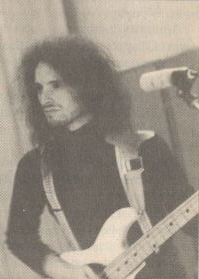
\includegraphics[scale=0.9]{Image09}
    \caption{\textit{Алик Грановский}}
\end{wrapfigure}

Работа Владимира Холстинина с «Волшебными Сумерками» к тому времени уже закончилась, и теперь он вместе со своим старым
другом Виталием Дубининым трудился в «Альфе» Сергея Сарычева. Они записали альбом и сделали попытку устроиться на работу
в Москонцерт. Но тарификационная комиссия, дававшая в те времена разрешение музыкантам на публичное исполнение песен,
крайне негативно отнеслась к группе Сарычева, и основное их неприятие вызвала песня «Московский озорной гуляка»,
написанная на слова Сергей Есенина, — та самая песня, что сделала «Альфу» сверхпопулярной среди простого народа. Но
какое дело худсовету до мнения простых народных масс? Запретить — и все тут!

Таким образом «Альфа» в 1983 года осталась без работы, из-за чего бас-гитарист Виталий Дубинин и барабанщик Сергей
Сафонов покинули Сарычева и ушли на заработки. Тогда-то Холстинин в надежде сохранить группу позвонил Грановскому и
пригласил его в «Альфу». Он же разыскал и нового барабанщика Игоря Молчанова. Однако и этому составу не суждено было
найти работу в филармониях.

Время шло. Деньги, привезенные Грановским из Карелии, подходили к концу, а ведь Алику было уже 23 года, у него уже
имелась семья, и он понимал, что необходимо искать, как заработать деньги. Да и музыка «Альфы», опирающаяся в первую
очередь на клавиши и ориентированная на поп-рок, казалась Грановскому чужой. Вот «Смещение» — это был настоящий
«тяжелый» рок!

Тогда-то Грановскому позвонил товарищ, которого он знал с детства, барабанщик Саша Воловик, и сказал, что есть работа в
Казахстане: создается бригада для концертного «чеса» по поселкам: «Можно поехать заработать денег, — а через три месяца
вернуться». Алик вызвонил в Петрозаводске Крустера: «Приезжай, меня вызывают в кокчетавскую филармонию, поехали
вместе!». — «Здорово! — прокричал сквозь плохую слышимость Андрей, — я скоро буду! Жди меня!».

Казахстан в то время являлся настоящим Эльдорадо для рок-музыкантов. За три-четыре месяца гастрольного «чёса» оттуда
можно было вернуться домой с деньгами, так необходимыми для покупки приличного инструмента или полного комплекта
гитарных эффектов. Правда, играть зачастую приходилось в совершенно фантастических условиях, когда сценой становилась
бескрайняя, овеваемая ветрами, степь, а зрительный зал заменяли два десятка стульев, выставленных из юрт. Да и жилищные
условия для музыкантов были отвратительными: чаще всего — «Дом колхозника» с удобствами во дворе. Но набитый денами
гитарный кофр сполна окупал все эти неудобства\ldots

Гастроли Крустера по Карелии затянулись, и он вернулся в Москву в тот самый день, когда необходимо было садиться на
поезд, отправлявшийся в Кокчетав. Но Андрей настолько устал в карельских гастрольных передрягах, что едва дойдя до дома,
рухнул совершенно обессиленный. Грановский отправился в Казахстан один. Пожалуй, если бы они тогда не расстались, то
играли бы вместе до сих пор. Но судьба распорядилась иначе.

Андрей Крустер снова уехал в Петрозаводск, где сломал руку и не смог больше играть на гитаре. Однако к тому времени он
уже настолько освоился в местной филармонии, что решил занять административный пост, в перспективе стать директором
филармонии и создать в Карелии райский край для рок-н-ролльщиков. (Надо сказать, что он добился своего и поднялся по
этой служебной лестнице почти до самого верха. Но совсем не вовремя началась «перестройка», и оказалось, что весь его
героический труд был напрасен, потому что сама жизнь дала рок-музыке «зеленый свет».)

Вернувшись из трехмесячной поездки по Казахстану. Грановский позвонил своему приятелю Сергею Потемкину, и тот аж
закричал в трубку: «Тут мой знакомый Коля Носков собирает группу, я — гитарист, он — вокалист, приезжай быстрее!».

Они сидели у Потемкина дома и часами разговаривали, какую будут играть музыку, но ничего не делали вообще. Однажды
пришел Носков и сообщил друзьям, что познакомился с Виктором Яковлевичем Векштейном, руководителем ВИА «Поющие Сердца»,
и тот предложил создать рок-группу, первую официальную рок-группу в Москонцерте. Они пришли, прошли прослушивание
и\ldots стали музыкантами ансамбля «Поющие сердца».

\begin{figure}
    \centering
    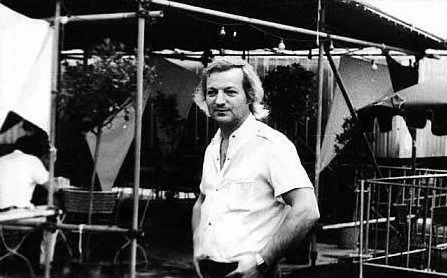
\includegraphics[scale=0.9]{Image10}
    \caption{\textit{Виктор Яковлевич Векштейн}}
\end{figure}

Векштейн предоставил для работы великолепную репетиционную базу, на которой стоял полный комплект крутейшей по тем
временам аппаратуры «Динаккорд», и они начали сочинять какие-то песни, но\ldots Недели через две Векштейн пришел и
сказал: «Хватит! Теперь начинается настоящая работа». Размечтавшимся рокерам раздали партитуры и доходчиво объяснили,
что они будут аккомпанировать жене Векштейна — певице Антонине Жмаковой. Ничего другого им не оставалось делать, потому
что они уже получали зарплату у Векштейна. А вскоре к Носкову, Потемкину и Грановскому присоединились Кирилл Покровский
(клавиши) и Александр Львов (барабаны), а затем вполне уже боеспособный состав после короткого репетиционного периода
отправился на гастроли.

Концерт состоял из двух отделений: в первом отделении исполнялись две песни Носкова, пара вещей Векштейна и какая-то
инструментальная музыка, во втором — этот же состав аккомпанировал Антонине Жмаковой. Никаким роком, естественно, и не
пахло, и вскоре Носков, которому осточертело исполнять эстрадную муть, разругался с Векштейном и покинул группу. На
освободившееся место вокалиста был приглашен Валерий Кипелов, один из солистов ВИА «Лейся, песня», только что
расформированного по решению тарификационной комиссии.

Как-то вечером Грановскому позвонил Холстинин.
— Привет, Алик! Как дела? — спросил он.
— Да вот, играю в «Поющих сердцах».
— Не нужен ли вам второй гитарист?
— Да, в общем-то, второй гитарист нам нужен, — ответил Алик. — Приезжай, может, и сгодишься.

Холстинин приехал, проиграл что-то по нотам — и его взяли. Некоторое время «Поющие сердца» ездили с двумя гитаристами —
Потемкиным и Холстининым. Говорят, из зала было забавно смотреть на эту пару. Потемкин роста был маленького, к тому же
играя он постоянно приседал и пригибался. Вместе с более высоким Холстининым они смотрелись как Пат и Паташон! Но этот
тандем просуществовал очень недолго. Хотя Потемкин был «сильным» гитаристом, Векштейн собирался его уволить и уже искал,
кем бы его заменить. Сергей и сам понял, что его дни в коллективе сочтены, и ушел не дожидаясь отставки. А ушел он
именно в «Альфу», наконец-то принятую на работу в филармонию.

Таким образом в «Поющих сердцах» сложился состав, который и станет первым составом будущей «Арии»: Кипелов, Холстинин,
Грановский, Львов и Покровский, — собственного материала они тогда еще не создали, но очень этого хотели\ldots

\begin{figure}
    \centering
    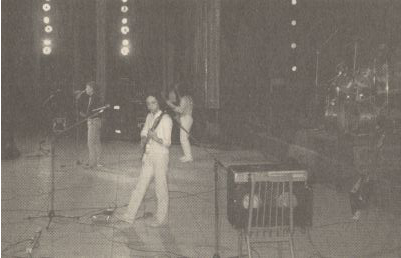
\includegraphics[scale=0.8]{Image11}
    \caption{\textit{
        ВИА «Поющие Сердца» до прихода Холстинина. Поет уже Валерий Кипелов, на гитаре играет Сергей Потемкин, на басу -
        Алик Грановский, за барабанами - Александр Львов
    }}
\end{figure}

Андрей Большаков и Александр Елин в это время трудились над проектом «Зигзаг». Андрей тогда увлекся музыкой «Jam»,
«Clash», Дэвида Бирна (David Birn), и пытался синтезировать это авангардное направление «новой волны» с хард-роком. Елин
довольно быстро написал абсолютно фантасмагоричные, но весьма адекватные этой странной музыке тексты. Там встречались
интересные песни — «Суета сует», «Где же ты, Ной?», «Телевидеобум» — вполне отвечавшие духу эпохи.

\begin{wrapfigure}{L}{0.5\textwidth}
    \centering
    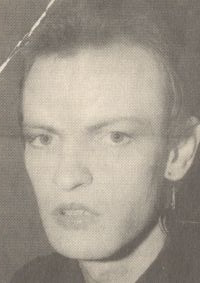
\includegraphics[scale=0.9]{Image12}
    \caption{\textit{Большаков периода «Зигзага»}}
\end{wrapfigure}

Когда репертуар был создан, стал вопрос о набор состава. Через некоторое время к Большакову присоединились бывшие
музыканты «Коктейля» Бутузов и Шатуновский, а следом клавишник Александр Вахмистров. Вскоре, правда, Шатуновский ушел, и
его заменил барабанщик Павел Чиняков, игравший до этого в «Альянсе». Впоследствии место за ударной установкой занял
Виктор Калашников (в дальнейшем. «Черный Кофе» и «Родмир»), а Чиняков переместился за бонги и конги. Собирая «Зигзаг»,
Большаков твердо решил найти вокалиста, но так и не смог подобрать певца, который в одинаковой степени сумел бы петь и
эмоционально, и прикольно, как пели панковские команды. Возможно, петь так тогда в СССР не умел никто. И пришлось
Большакову снова петь самому: «Во времена «Зигзага» я ставил волосы «ежиком» и заклеивал передние зубы черной изолентой,
чтобы придать себе вызывающий вид\ldots»

«Зигзаг» начал с записи альбома, сразу попавшего к подпольным «писателям», и их усилиями оперативно распространившегося
по всей стране. А вот концерт в истории группы состоялся лишь один — в актовом зале какого-то министерства на улице
Лубянке. Сразу после этого вышло постановление министерства культуры СССР, запрещавшее концертную деятельность многих
групп, и «Зигзаг» стоял в самом начале этого «черного списка». Ушедший из «Зигзага» Андрей Шатуновский предложил своим
друзьям выход из ситуации: «Ребята, — сказал он, — у меня есть друг Валера Левушкин, руководитель ансамбля «Бим-Бом». У
них база на Пушкинской. Туда можно пойти, чтобы сохранить команду. Можно работать в «Бим-Боме», а параллельно игры свою
музыку». Левушкин радостно откликнулся на это предложение, так как музыканты «Зигзага» являлись настоящими
профессионалами — бросаться такими было нельзя.

Надо сказать, что ансамбль музыкальной пародии «Бим-Бом» тогда очень много выступал, принося своим участникам и деньги,
и заграничные поездки, но заниматься собственным творчеством там оказалось совершенно невозможно, так как репетиции и
гастроли занимали абсолютно все время. Большаков выдержал лишь год подобной жизни, а потом покинул «Бим-Бом»\ldots

\begin{figure}
    \centering
    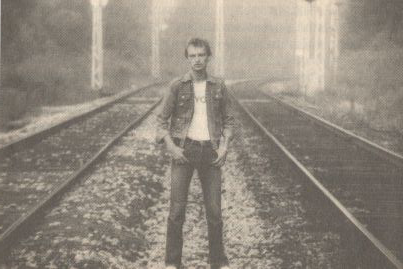
\includegraphics[scale=0.9]{Image13}
    \caption{\textit{Большаков времен альбома «Надоело»}}
\end{figure}

В этот самый момент Андрей сидел дома один-одинешенек и мрачно размышлял о том, насколько здорово было бы работать в
профессиональной группе, исполняющей рок-музыку, да еще бы всю эту музыку писать самому!.. Но, видно, не судьба — да и
времена какие-то совсем не рок-н-ролльные. А тут еще за окном осенний дождь зарядил, и вообще холодная погода нагрянула
так внезапно, хотя еще вчера вокруг царило лето и светило теплое солнышко. Постепенно горькие мысли начали превращаться
в музыку, но не в «тяжелый» рок (что казалось правильным), а в светлые и немного печальные мелодии. На огонек заглянул
Саша Елин. Он прислушался к звукам, что рождались на гитарных струнах, и они вдохновили его на целый цикл текстов, в
которых затрепетали понятные каждому из соавторов чувства. Позже эти песни прозвучали на альбоме «Надоело», записанном
Большаковым с помощью простенькой драм-машины да безымянного ныне клавишника, игравшего фоновые подкладки песен\ldots

А в это время будущие «арийцы» тоже поняли, что им нужен новый репертуар, который необходимо записать в виде альбома.
Получив от Векштейна «добро» на использование его шикарной 16-тиканальной студии, Грановский с Холстининым заперлись на
квартире у Володи, и за неделю сотворили первую музыкальную программу. Однако предстояло еще найти поэта, способного
создать нужный текст, и задача эта была не простой ввиду того, что все профессиональные поэты того времени писали для
вокально-инструментальных ансамблей и в их сознании уже царствовали штампы этого выхолощенного жанра. Было понятно, что
для «тяжелого» рока нужна «свежая» идея. Друзья Векштейна посоветовали ему пригласить поэтессу Маргариту Пушкину,
известную интересными работами с группами «Високосное лето» и «Автограф». Знакомые Владимира Холстинина обратили
внимание на Александра Елина, создававшего тексту для «Альянса», «Зигзага» и «Гулливеров».

Елин в то время лежал в больнице с гепатитом, и кассету с «рыбой», то есть музыку с напетым псевдо-английским текстом
ему передали через жену. У кого-то из соседей по больничной палате имелся магнитофон, и как только Саша вставил кассету
и включил ее, он мгновенно понял, что наконец слышит то, о чем мечтал уже много лет. Буквы сами начали слагаться в
строки песни. Первым материализовался текст песни «Это — Рок» (песня станет первой и на альбоме), затем — «Бивни Черных
Скал», а за ними рвалась на бумагу Жизнь задаром»\ldots Когда Елин выписался из больницы, он сразу же отправился на
студию Векштейна в Хамовниках. Там и состоялось знакомство Елина с Холстининым и Грановским, и все они друг друга
внимательно осмотрели и буквально «обнюхали», потому что понимали всю ответственность творческого союза, в результате
которого должен был родиться первый альбом «Арии».

Грановский спросил у Елина, нет ли у него на примете хорошего гитариста — к тому времени Потемкин ушел из группы. На
альбоме все гитарные партии записал Холстинин, а для гастролей требовался второй гитарист. Елин ответил, что у него есть
человек, который сыграет все, что угодно.

Тем же вечером Елин заскочил к Большакову. «Знаешь, Саша, пока ты болел, — встретил друга Андрей, — я надумал снова
собирать группу!». Его горящие глаза выдавали мрачную решимость воплотить сказанное вопреки любым препятствиям.

— А ты не хочешь пойти в «Поющие Сердца»? — спросил Елин. — Я с ними сейчас как раз работаю.
— А что они играют?
— А они играют металл! — и Елин поставил на магнитофон заготовку песни «Волонтер».
— Какой класс! — только и смог вымолвить Большаков.

На следующий день Елин привел Большакова на базу «Поющих Сердец» в ДК имени Фрунзе. Присутствовал один Грановский, и
когда Андрей с Аликом посмотрели друг другу в глаза, будто искра проскочила меж ними. В ожидании Векштейна они поиграли
какие-то риффы, поговорили о том, кто что любит, тут приехал Виктор Яковлевич, спросил у Грановского, как ему показался
новый гитарист, и, услышав положительный ответ, кивнул Большакову: «Ладно! Мы тебя берем! Завтра приезжай в Москонцерт с
документами оформляться». Но эти слова являлись завершающей формальностью, истинная магия совершилась раньше.
\textbf{Подобный момент специалисты-астрологи называют Точкой Сборки. С приходом Большакова не только окончательно
сформировался первый состав «Арии», но и костяк будущей группы «Мастер»\ldots}

Внимательный читатель уже должен был заметить, что Грановского с Большаковым фактически познакомил не кто иной, как
Володя Холстинин, а это означает, что системного конфликта между Большаковым и Холстининым, как его описывают в книгах,
не было. Что же происходило на самом деле? «Ария» стала инкубатором для «Мастера», но ведь группа должна была как-то
вылупиться из яйца, поэтому все скандалы и разборки в «Арии» являлись тем самым «тут-тук-тук», которым цыпленок
пробивает себе дорогу на волю\ldots

Большаков успел принять участие в записи первого «арийского» альбома, но не как гитарист, а как бэк-вокалист. А когда
«Поющие Сердца» отправились на очередные гастроли, выяснилось, что «тяжелого» материала для полноценного отделения
продолжительностью в час не хватает. Тогда Холстинин и спросил Андрея, нет ли у него в запасе каких-нибудь композиций,
которыми можно было бы дополнить программу?

— Конечно, есть! — ответил Большаков.
— Так неси скорее!

Первым произведением, которое Андрей Большаков принес «Арию», была композиция «Икар», написанная еще во времена
«Коктейля», но не входившая в основной репертуар. в «Арии» она была аранжирована в стиле «Iron Maiden», как того хотел
Холстинин. Песня «Без тебя» также была старой песней Большакова, написанной для сольного альбома, куда она так и не
вошла. Кипелов немного скорректировал ее мелодию и куплет, поэтому авторство на музыку стало общим: Кипелов — Большаков.
Следом была сочинена песня «Воля и разум», затем — «Встань, страх преодолей!». Рифф песни «Встань, страх преодолей!» был
навеян композицией группы «Saxon» с альбома 1984 года, который Большаков однажды слушал вместе с Грановским, но сама
гармония и даже гитарное соло были позаимствованы из песни «Мы принимаем передачи», написанной Андреем во времена
«Зигзага». Все новые композиции сразу же были включены в концертную программу.

После гастролей в Новгороде штатный барабанщик «Пoющих Сердец» Александр Львов из-за ударной установки пересел за
звукорежиссерский пульт. На освободившееся место был приглашен Игорь Молчанов, с которым Холстинин и Грановский когда-то
играли в «Альфе».

\textbf{Как только собрался данный состав, и был создан репертуар, должен был раздаться сигнал «тук-тук-тук», извещающий
о том, что птенец «Мастер» готов выбраться из яйца на волю. Это событие произошло во время гастролей группы в городе
Владимире.}

В зале владимирской филармонии шла обычная репетиция, как вдруг Векштейн подошел к Алику Грановскому и сказал: «Алик, у
тебя такие длинные волосы, ты их убери лучше куда-нибудь, а то нас могут закрыть. Напишут еще, чего доброго, телегу в
Министерство культуры — и до свиданья. Здесь все очень строго, поэтому мы решили, что ты их будешь куда-нибудь убирать».
Но Грановский — рокер в полном смысле этого слова, он прошел испытание настоящим андеграундом. Бояться после этого
доносов — нонсенс, а тут от него еще требуют прогибаться! Разумеется, он очень напрягся. «Тогда, Алик, ты будешь играть
за кулисами, — продолжал наезжать Векштейн, — сядешь там на стульчик, распустишь хаера! А вместо тебя мы поставим на
сцену какого-нибудь симпатичного парня!»

\begin{figure}
    \centering
    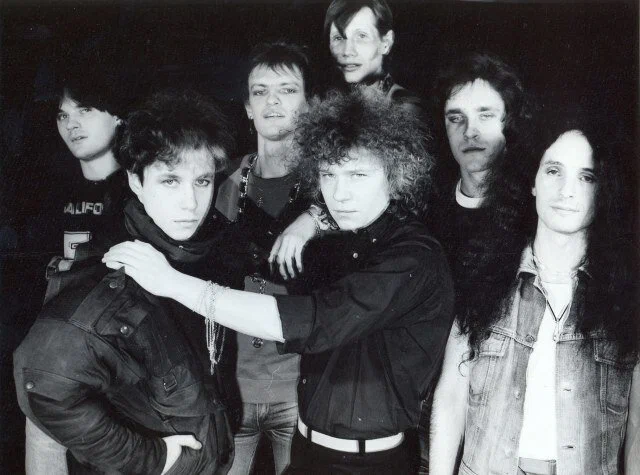
\includegraphics[scale=0.9]{Image14}
    \caption{\textit{
        «Ария»: Александр Львов, Кирилл Покровский, Андрей Большаков, Валерий Кипелов, Владимир Холстинин, Алик
        Грановский, позади всех - только пришедший в группу Игорь Молчанов
    }}
\end{figure}

Надо сказать, что Векштейн давно уже был недоволен длинными волосами Грановского, он постоянно пенял Алику: «В
Москонцерте не может быть такого хаера!». Да, иметь подобную длину волос в государственной организации, которой в полной
мере являлась филармония, было в те времена не принято, и, возможно, руководители филармонии требовали от Виктора
Яковлевича, чтобы он подстриг своего артиста. И если до сих пор Алику удавалось все эти наезды обращать в шутку, то на
сей раз он вспылил: «Чуваки, ну что за дела?! Валить отсюда надо и делать свою группу!».

Грановский подошел к Холстинину, ища сочувствия и поддержки, а тот сказал, медленно и очень веско: «Уходи! А мы будем
искать другого басиста».

«Володя, а ты меня спросил? — вмешался в конфликт Большаков. — Лично я уйду вместе с Аликом! Ты будешь искать не только
нового басиста, но и нового гитариста!..»

Векштейн почувствовал, что возникшее напряжение выводит ситуацию из-под контроля, и сразу нажал на тормоза: «Так,
репетиция заканчивается! — скомандовал он. — Все быстро в гостиницу, а там — ко мне на разговор!» Когда все собрались у
него в номере, Виктор Яковлевич дипломатично разрядил обстановку: «Алик, я же пошутил. Работаем дальше\ldots».

Нужно сказать, что ничего кардинального в тот момент произойти просто не могло — сама группа «Ария» тогда еще фактически
не существовала, цыпленку просто неоткуда было вылупиться. Это был вокально-инструментальный ансамбль «Поющие Сердца»,
просто в первом отделении пела Антонина Жмакова, а во втором исполнялись песни из «металлического» репертуара.

Векштейн постарался взять ситуацию под жесткий контроль, так как ему вовсе не хотелось терять такой мощный творческий
тандем, каким был союз Грановского Большакова, ведь они написали большинство «арийских» хитов. К тому Большаков по
просьбе Векштейна сочинял песни для Антонины Жмаковой. После долгих раздумий Векштейн решил принять сторону Андрея и
Алика. Когда «арийцы» как-то раз закончили репетировать, Векштейн позвал всех погулять — в Парке Горького был небольшой
стадион, и они часто ходили вокруг него и подолгу беседовали о разном. На ту прогулку пошли все, кроме Холстинина и
Кипелова. И там Векштейн объявил Грановскому и Большакову, что принимает все их условия: «Iron Maiden» уже неактуальны,
уже появилась «Metallica», и нужно играть, как они». «Я ставлю на вас», — подвел итог разговору Векштейн.

В феврале 1986 года Векштейн дал разрешение на запись нового альбома. Большаков и Грановский две недели дневали и
ночевали в студии, а под завершение работы Андрей позвонил Холстинину и попросил его приехать и сыграть свои партии
соло, чтобы на записи звучали разные гитаристы. Так тогда было принято и в «Iron Maiden», и в «Judas Priest» — чтобы
гитаристы играли по очереди: кусочек один, следующий кусочек — другой, а на конвертах пластинок обычно указывалось,
какое соло исполняют Типтон и Даунинг, а какое — Смит и Мюррей. Володя приехал, молча все записал и уехал. Это были соло
песнях «Воля разум», «Игры не для нас».

У самого Холстинина к тому времени уже была написана песня «Тысяча сто», но для нового студийника он ее предлагать не
торопился, потому что альбом «С кем ты?» был совсем не похож на предыдущий альбом, скорее это являлось студийной работой
какой-то иной группы, на современном языке можно сказать, что это был виртуальный альбом несуществующей еще группы
«Мастер». Действительно, музыкальный стиль поменялся, он стал более жестким и агрессивным и совершенно иным, чем
творчество группы «Ария», как до, так и после этого альбома. Даже название альбома — «С кем ты?» — говорит о том, что
это была попытка нескольких музыкантов идентифицировать себя как некую новую формацию, недаром Холстинин на записи играл
лишь роль сессионного гитариста.

Любопытно, что во время работы над вторым альбомом база «Арии» и студия Векштейна переехали из Хамовников в Парк
культуры имени Горького, где тогда репетировала группа Сергея Потемкина «Форт-Росс». Но после того как Большаков и
Грановский со-товарищи ушли из группы, «Ария» вновь вернулась в Хамовники, правда, не в легендарный офицерский ДК имени
Фрунзе, а в ДК имени Свердлова, расположенный неподалеку от Новодевичьего монастыря. (Там позже будет записан альбом
«Герой асфальта».)

\begin{figure}
    \centering
    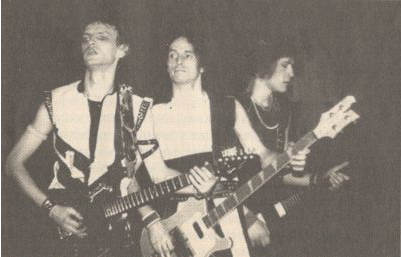
\includegraphics[scale=0.8]{Image15}
    \caption{\textit{Бальшаков, Грановский и Холстинин в составе «Арии»}}
\end{figure}

Холстинин ходил тогда совершенно потерянный, явно не понимая, что предпринять в сложившейся ситуации. То страшное
напряжение, которое тогда существовало в «Арии», казалось, можно было потрогать руками. Владимир даже хотел покинуть
группу, потому что ощущал себя лишним и одиноким. Возможно, если бы он это сделал, то «Ария» стала бы играть «трэш», и
история пошла бы иным путем. Но этого не произошло, потому что на какое-то время Володя Холстинин стал рукой Судьбы.

\ldotsИменно Грановский и Холстинин осенью 1986 года уговорили Векштейна изменить название «Поющие Сердца» на «Арию». К
тому времени первый альбом «Арии» «Мания величия» усилиями писателей разошелся по стране, и, куда бы ни приезжали
«Поющие Сердца», повсюду их ожидали аншлаги и бешеный успех, так как «металлическая» музыка именно в тот момент была
крайне популярна. Векштейн давно уже убедился в том, что «металлическую» программу публика принимает значительно лучше,
чем эстрадную, но на эксперимент он решился исключительно под постоянным прессингом Алика и Володи.

«Поющие Сердца» должны были выступать в украинском городе Черновцы, и Векштейн отправил туда афиши, на которых впервые
значилось «Ария» (их везде уже знали как «Арию»). И вот музыканты приезжают в филармонию, завешенную афишами с гордым
именем «Ария», и тут Векштейн приглашает всех к себе в номер и объявляет: «Меня вызывают в Москву. Кто-то уже
накапал\ldots». Этого и следовало ожидать, ведь разрешение на официальные выступления имел вокально-инструментальный
ансамбль «Поющие «Сердца», а вовсе не «хэви-металлическая» группа «Ария». За самовольное изменение названия в ту пору
следовало моментальное расформирование коллектива. И местные филармонические боссы накатали «телегу» в Москву, так как
отлично понимали, что, пропусти они выступление группы с неутвержденным названием, их самих могли бы уволить с
насиженных теплых местечек.

Итак, Векштейн уехал в Москву, а музыкантов поселили в закрытом лесном пансионате для партийных работников. Поскольку
сидеть сложа руки было скучно, Большаков, Грановский и Молчанов ездили в филармонию и в комнатке, где стояла их
аппаратура, репетировали новые вещи. В Черновцах были созданы песни «Щит и меч» и «SOS», которые позже вошли в репертуар
будущей группы Большакова и Грановского. Это уже была попытка перейти от стилистики «Iron Maiden» и «Judas Priest» к
«трэшу». Приехать на репетиции было предложено и Кипелову с Холстининым, но те отказались (ведь это была уже не «Ария»,
а «Мастер», пусть пока не имеющий ни статуса, ни названия).

А потом вернулся Векштейн и объявил, что дела плохи: придется возвращаться в Москву и сдавать программу. «Но сдавать ее
надо, чтобы нам утвердили название «Ария»\ldots», — сказал Виктор Яковлевич. Вскоре в Москве состоялся тот знаменитый,
описанный во многих книгах худсовет, на котором Векштейн сумел убедить руководство Москонцерта, что новый молодежный
«хэви-металлический» коллектив даст Москонцерту больше прибыли, чем традиционный ВИА «Поющие Сердца». В итоге разрешение
на гастроли было получено, и в следующую поездку группа отправилась уже как «Ария».

\textbf{\ldotsТолько теперь, когда «Ария» наконец обрела свое имя, птенец мог разбить скорлупку и выбраться из яйца. Это
и произошло во время гастролей «Арии» в Ставрополе\ldots}

На концерте «Арии» в Ставрополе зал был заполнен отказа, и уже на второй песне возбужденные зрители полезли на сцену. Но
Ставрополь — родина тогдашнего руководителя страны Михаила Горбачева (по совместительству занимающего пост генерального
секретаря всесильной коммунистической партии СССР), поэтому шуметь там не полагалось, а «металл» и вовсе был чужеродным
элементом. Напуганный Векштейн приказал отключить аппаратуру от электричества и потребовал, чтобы зрители сели на свои
места. Виктор Яковлевич ужасно боялся, что в Москву из Ставрополя уйдет письмо, после которого его группу, его любимое
детище расформируют\ldots

Когда музыканты вновь начали играть, публика опять вскочила со своих мест, и Векштейн опять выключил звук. Тогда все
музыканты, за исключением Холстинина, ушли со сцены. Векштейн прибежал за кулисы, стал кричать и требовать, чтобы
участники группы вышли на сцену и продолжили концерт. В кульминационный момент он схватил Грановского за грудки и
попросту вытолкнул его на сцену\ldots

В каком-то смысле Векштейна можно понять. Поясним, что в те времена взаимодействие художественного руководителя с
музыкантами весьма походило на взаимоотношения Карабаса Барабаса с его деревянными куклами. По мнению Векштейна, его
куклы были в этом случае просто неблагодарными деревяшками. Он обеспечивал им высокий заработок, классные инструменты и
аппаратуру, предоставлял студию для записи, а также право официально исполнять на сцене о любимую «тяжелую» музыку. Ради
этого можно стерпеть такую мелочь, как хозяйский окрик. А если кто-то недоволен — «скатертью дорога»! По улицам бродит
куча безработных кукол, готовых прибежать, стоит их только пальцем поманить!.. В общем, времена были другие\ldots В
итоге музыкантам все же пришлось выйти на сцену и довести концерт до конца. Но подобное выступление «из-под палки» еще
больше усилило напряжение в группе.

Вечером того же дня состоялось собрание, на котором Грновский, Покровский, Большаков и Молчанов заявили Векштейну, что
собираются уходить. Виктор Яковлевич сражался до последнего патрона, а когда боезапас иссяк, оказалось, что он готов
пойти на значительные уступки. «Так что вас не устраивает?» — спросил он в конце концов.

— Нас не устраивает все! — ответил Большаков.
— Нет, это не разговор. Давайте конкретно, по пунктам.
— Нам надоело ездить по «овощному кольцу». Великие Луки, Малые Луки — сколько ж можно? — ввязался в диспут Грановский.
— Алик, проблема решена, — сказал Векштейн. — Мы не будем больше ездить по «овощному кольцу». Что-то есть еще?
— Да! Нам бы хотелось работать в Москве!
— Хорошо, мы работаем в Москве. Дворец спорта вас устроит?
— И чтобы волосы не прятать!!!
— Теперь можно не прятать.
— А цепи?
— И цепи можно одевать. Это все, что вас не устраивает?
— Все!
— Ну, вот мы все и решили. Прямо сейчас, — подвел итог разговору Векштейн. Его задача была одна: расколоть группу на
части, чтобы потом без помех уволить неподдающегося Грановского. Но Большаков поддержал своего друга. Почувствовав, как
Векштейн постепенно забирает контроль над ситуацией в свои руки, он вскочил со своего места и заявил: «Виктор Яковлевич,
не знаю, как другие, но я все равно уйду с Аликом!».

Молчанов тут же предложил пересчитать всех, кто остается, и оказалось, что остаются только Холстинин и Кипелов.

Когда группа вернулась в Москву, Векштейн действительно договорился о концертах «Арии» в Лужниках, в спортзале «Дружба»,
которые и состоялись в начале января 1987 года. В Москве стоял жуткий мороз, но народ стоически переносил невзгоды: от
метро «Спортивная» ко Дворцу спорта двигался нескончаемый людской поток, подъезжали и подъезжали автобусы с фанами,
приехавшими из провинции, а те, кому не досталось заветного билетика, уже в метро встречали счастливчиков написанными от
руки плакатами: «Куплю билеты на «Арию»\ldots». Несмотря на то, что и в Москве, и в Питере было уже довольно много
известных команд, играющих «тяжелую» музыку, например «Черный Кофе», «Металлаккорд» или «Август», они выступали в
маленьких залах, а тут — «хэви-металлические» концерты в Дворце спорта. В Москве подобное происходило впервые. Эта
музыка до того времени жила в подполье, и на официальных площадках, вмещающих больше тысячи зрителей, таким группам
просто не давали работать. Наблюдая предконцертный ажиотаж, Большаков сказал Грановскому: «Знаешь, это – наш с тобой
последний концерт в «Арии», давай выложимся по полной программе!» И они отыграли на «пять с плюсом», при этом устроили
настоящее шоу — носились, прыгали, «отвязывались» как могли.

Была ли у Векштейна возможность оставить в «Арии» уходящих от него музыкантов? Пожалуй, нет. Тем более что Холстинин на
концерты в «Дружбу» уже пригласил музыкантов, которые должны были заменить Большакова, Грановского и компанию. Это были
гитарист Сергей Маврин и барабанщик Максим Удалов, а также старый друг Холстинина по «Волшебным сумеркам» бас-гитарист
Виталий Дубинин. С их приходом в группу и начнется истинное «арийское» время, недаром именно этот состав «Арии»
считается «золотым»\ldots

Лейтмотивом 1987 года стал лозунг: «выйти из-под контроля», и питерская группа «Телевизор», получившая популярность в
первую очередь благодаря актуальным текстам, даже сочинила хит с таким названием. Это было время, когда рок-музыка вышла
из подполья, время борьбы с властью, время создания новых концертных организаций (рок-клубов и рок-лаборатории) как
альтернативы государственным филармониям. Векштейн, которого с трезвых позиций сегодняшнего дня можно считать гениальным
создателем группы, рост популярности которой продолжается уже более пятнадцати лет, тогда однозначно считали Врагом
Номер Один и Богатеньким Дядечкой, наживающимся на талантливых музыкантах, а поэтому расставание с ним было исторически
предрешено. Отметим, что расстанутся с Векштейном не только раскольники, создавшие группу «Мастер», но и — спустя чуть
более года — сама группа «Ария»\ldots

Грановский с Большаковым были не единственными, кто тогда покинул родную группу. Вскоре Дмитрий Умецкий оставил
«Наутилус Помпилиус», Жанна Агузарова в первый раз ушла из «Браво», Виктор Троегубов впервые покинул «Крематоpий», чуть
позже Анатолий Крупнов и Петр Мамонов объявили о расформировании «Черного Обелиска» и «Звуков МУ», а Борис Гребенщиков и
вовсе катапультировался в Америку. Просто «Ария» была первой в длинной череде распадов и расставаний.

В том же году где-то за океаном группа «Aerosmith» вышла из-под власти наркотиков и вернулась в таблицы популярности.
Дэвид Ли Рот (David Lee Roth) ушел от Эдди Ван Халена (Eddie Van Halen). Гитарист Джон Норум (John Norum) ушел из группы
«Europe» и основал собственный коллектив. Из «Black Sabbath» ушли Батлер (Geezer Butler) и Ворд (Bill Ward), и Йомми
(Tony Iommy) реализовал новую пластинку как сольный проект\ldots Распались «Twisted Sister», «Metallica» едва не
развалилась из-за гибели Клиффа Бартона (Cliff Burton), «Der Leppard» выпустил знаменитый диск «Hysteria», «Megadeth»
обозначил главный курс «трэша» альбомами «Peace Sells\ldots But Who's Buying?» и «So Far, So Good\ldots So What?»\ldots

Надо сказать, что «Мастер» уходил вовсе не в безвоздушное пространство. Перед тем как покинуть Векштейна, Большаков
встречался с Валерием Гольденбергом, администратором Московской областной филармонии, который организовывал стадионные
концерты для групп «Браво», «Рондо» и проекта Константина Никольского «Зеркало мира». Однажды Гольденберг решил сделать
большую концертную программу на все вкусы. К «Браво» и «Рондо», исполнявшим разные виды «нью-вэйва», и Константину
Никольскому, который ориентировался на традиционный хард-рок, он задумал добавить «хэви-металлическую» команду.

Гольденберг был именно тем человеком, котором тогда нуждалась группа «Мастер». Во-первых, его авторитет в шоу-бизнесе
был непререкаем, а во-вторых, он не вмешивался в творчество, как это делал Векштейн. «Ну что вы мне все твердите: музыка
да музыка! Меня совершенно не интересует, что вы играете. Но если ваша музыка продается, я буду ее продавать\ldots —
сказал Гольденберг Андрею. — Все, что я могу для вас сделать, это зарядить столько концертов, сколько вы сможете
отыграть. Сколько вы можете работать концертов в месяц?»

— Что значит, сколько мы можем? — удивился Большаков.
— Вот сколько сможете, столько и будете работать.
— Такого не бывает! — ответил Андрей.
— Еще как бывает! — словно отрезал Гольденберг\ldots

Не откладывая в долгий ящик, он начал звонить в другие города и договариваться о концертах.

— Все нормально, — сообщил он вскоре Андрею. — Готовьтесь!

Большаков не верил своим ушам. В «Арии» они работали в лучшем случае восемь концертов в месяц, а Гольденберг выстроил их
маршрут таким образом, что уже в первый месяц выпадало тридцать концертов. Причем все концерты — в центральных городах.

Гольденберг определил сроки, приобрел для группы нужные инструменты и аппаратуру, а также снял репетиционную базу в
подвальном помещении одного кунцевского ЖЭКа. Дело оставалось за малым: придумать новой группе название и
доукомплектовать состав для гастролей. Напомним, «Арию» покинул готовый инструментальный состав: басист, гитарист,
барабанщик и клавишник. Впрочем, так уж получилось, что как раз клавишник для той музыки, которую они собирались играть,
был не нужен. Поэтому Кирилл Покровский лишь иногда приходил на репетиции, и в основном занимался своим собственным
проектом. Зато новой группе не хватало второго гитариста и — самое главное — вокалиста\ldots

Гитарист был найден быстро: Игорь Молчанов привел своего друга Сергея Попова, который до этого играл в ВИА «Здравствуй,
песня». А вот вокалиста пришлось поискать. Сначала планировали пригласить Николая Носкова, но тому оказалась неинтересна
музыка «трэш». На прослушивание приходили певец группы «Новый завет» Вячеслав Горбачев и Гоша Корнеев, позже собравший
группу «Каре», но оба по разным причинам не подошли, хотя Большаков с Грановским отметили для себя, что Корнеев очень
профессионально пел перегруженным высоким вокалом в стиле «AC/DC»\ldots Когда поиски певца зашли в тупик, на помощь в
очередной раз пришел Сергей Потемкин, посоветовавший старым друзьям прослушать вокалиста Александра Арзамаскова, певшего
в группе Потемкина «Форт-Росс». Арзамасков покорил Большакова и Грановского тем, что без особого труда пел «в ноль»
любую песню с альбома «Burn», причем делам это на хорошем английском языке.

\begin{figure}
    \centering
    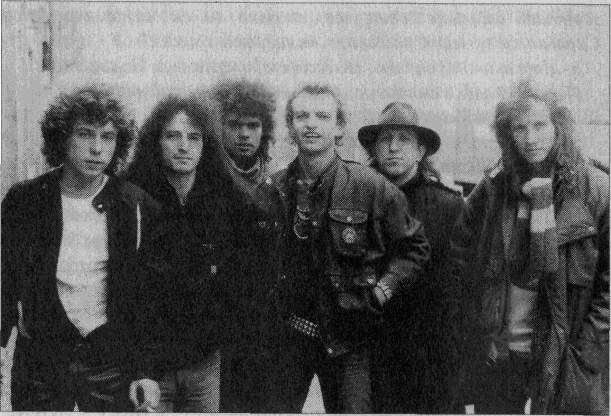
\includegraphics[scale=0.8]{Image16}
    \caption{\textit{«Мастер» №1: Покровский, Грановский, Попов, Большаков, Арзамасков и Молчанов}}
\end{figure}

Итак, состав был собран, теперь необходимо было придумать ему название. Как и полагается в таких случаях, музыканты
достали с книжных полок толстые словари и начали искать в них магическое слово. Вариантов рассмотрели немало, Большаков,
например, исписал с двух сторон целый лист. Хотелось чтобы название было одновременно и емким, и кратким, и что бы
запоминалось сразу, и чтобы внутренний подтекст присутствовал\ldots Решение пришло внезапно и в самом неожиданном месте.
Как-то раз Грановский с Молчановым возвращались после репетиции домой, и в метро, когда они уже подъезжали к станции
«Новокузнецкая», Игорь Молчанов предложил название «Мастер». Никакого скрытого смысла в нем не было, главное, чем это
название привлекло, — оно читалось одинаково на всех языках: наши герои уже тогда готовились покорять заграницу, Позже
досужие журналисты пытались как-то обыгрывать название, вспоминая роман Михаила Булгакова или древнее значение этого
слова, согласно которому Мастер — это человек, воспринимающий и воспроизводящий музыкальные послания свыше, как, скажем,
И.С.Бах, которого называли «маэстро», то есть «мастер». Алик всегда ругался, когда при нем заводили подобные разговоры:
«Обыграть это можно как угодно, и фабулу подвести можно любую, но я против этого», — говорил он. Когда же его
окончательно доставали рассуждениями о подоплеке названия группы, он рассказывал, что в 60-е годы по квартирам ходил
человек и «вырезал» людей: «Он звонил в дверь и представлялся мастером-водопроводчиком или мастером из Мосгаза. Вот он и
называл себя Мастером\ldots».

Векштейн узнав, что ушедшие от него музыканты назвали свою группу «Мастер», съязвил: «Какие же они мастера? Они —
подмастерья\ldots». Но сами музыканты, оставшиеся в «Арии», да и новые ребята, заменившие ушедших, буквально кожей
ощущали конкуренцию, все знали, что где-то к своему хитовому скачку готовится группа «Мастер», и желали только одного:
быть лучше их!

\begin{wrapfigure}{R}{0.5\textwidth}
    \centering
    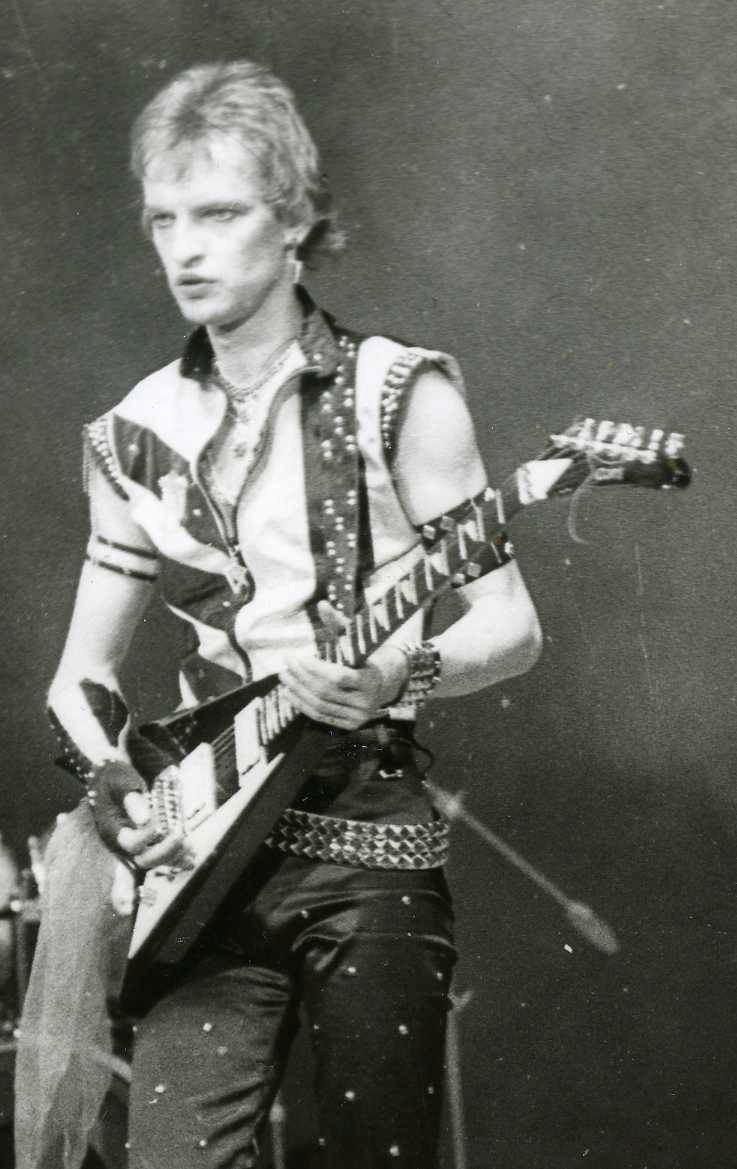
\includegraphics[scale=0.9]{Image17}
    \caption{\textit{Большаков: «Перед нашим первым концертом я купил гитару как у Рэнди Роудса\ldots»}}
\end{wrapfigure}

С оглядкой на «Арию» работали и музыканты «Мастера». «Я всегда следил за тем, что у них происходит и как происходит, мне
было важно это знать для разработки нашей политики: их ход — наш ход. Но я никогда не подавал виду, что меня это
интересовало, — открывает тайны ушедших дней Андрей Большаков, — наоборот, я всегда говорил только одно: «Ребята,
забудьте про «Арию»! Пока продолжается репетиционный период, мы должны существовать в своем собственном замкнутом
пространстве, потому что какими мы станем, такими нас публика и будет с ними сравнивать. Если мы ушли не зря и мы
чего-то достойны, то люди скажут: «Это круто» А если мы будем бить себя в грудь, а люди видят, что это не круто, значит,
мы ничего не стоим\ldots.».

Первая программа «Мастера» была составлена из песен с арийского альбома «С кем ты?». (Андрей Большаков сумел
договориться с Векштейном, что «Ария» не будет исполнять эти песни.) Кроме того, Большаков написал новые композиции
«Кто кого?», «Берегись», «Мастер» и «Храни меня», а Грановский принес в репертуар песню «Руки прочь».

Первый концерт «Мастера» состоялся 11 мая 1987 года в Ленинграде, в СКК «Юбилейный». Это не был сольный концерт группы,
«Мастер» работал в сборной программе «Молодые — молодым» вместе с «Рондо», «Браво» и «Зеркалом мира», но Гольденберг
абсолютно точно поставил наших героев в самый конец концерта, и «Мастеру» досталась львиная доля успеха. Давно уже
отгремел финальный аккорд «Воли и Разума», а публика в одиннадцать тысяч глоток продолжала, совершенно не уставая,
скандировать имя своих новых кумиров.

После концерта Большаков и Грановский шли по невской набережной, ночные огни отражались в Неве, плескавшейся в гранитных
берегах, и в этом мерном плеске музыканты слышали песню о весеннем преображении жизни.

\begin{figure}
    \centering
    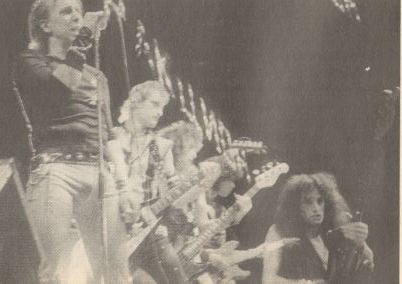
\includegraphics[scale=0.8]{Image18}
    \caption{\textit{Первый концерт «Мастера». Ленинград, 11 мая 1987 г.}}
\end{figure}

Андрей сказал тогда другу:

— Похоже, не зря мы ушли!
— Да, не зря! — откликнулся Алик\ldots

Спустя некоторое время появился еще один повод для радости — песня «SOS» попала в кинофильм «Ночной экипаж». На концерте
«Мастера» в московском Дворце спорта «Крылья Советов» в Сетуни побывал режиссер Токарев, безуспешно искавший для своего
нового фильма песню, несущую ощущение тревоги. (По сюжету фильма только что окончившие школу молодые люди угоняют такси,
милиция объявляет «охоту», а в итоге угонщики разбиваются — печальная история.) Режиссер выбрал песню «SOS», которая и
стала лейтмотивом этого фильма. Музыканты «Мастера» тоже попали в кадр: они сыграли роль музыкантов, выступавших на
выпускном вечере у тех ребят, которые потом украли автомобиль, и исполняли как раз песню «SOS»\ldots

Еще древние греки говорили, что лишь только подумаешь: счастлив, — как кончается счастье. В самый разгар гастролей у
Арзамаскова возникли проблемы со связками. Его голос был довольно низким, а первая программа «Мастера», созданная еще во
времена работы над альбомом «С кем ты?», была рассчитана на высокий голос Кипелова. Арзамасков чисто физически был не в
состоянии петь те ноты, которые Кипелов брал с легкостью, в результате сильного перенапряжения голосового аппарата он в
конце концов потерял голос. Врачи вынесли жесточайший вердикт: «Человеку не то, что петь – говорить нельзя!». В итоге
Арзамасков отработал с «Мастером» всего лишь месяц. За это время группа отыграла концерты в Питере, Твери, Москве (в
Центральном Доме Туриста) и Воскресенске, записала демо-альбом, куда вошли практически все вещи, что вышли потом на
пластинке, а также песня «SOS», вошедшая в кинофильм «Ночной экипаж». А вот июньские концерты в Воронеже из-за болезни
Арзамаскова пришлось отменить, и «Мастер» вернулся в Москву искать нового вокалиста.

В июле у Гольденберга был проложен маршрут по югу Украины: Николаев, Херсон, Запорожье и Скадовск, — поэтому на поиски
вокалиста и репетиции отводилось совсем мало времени, ведь Гольденберг не станет отменять гастроли из-за того, что
кого-то нет. Вот тут-то Грановский и Большаков и вспомнили про Гошу Корнеева, который приходил к ним на прослушивание.

— Ты помнишь, какой у него был высокий вокал? — говорил Грановский Большакову. — Уж для него-то взять высокие ноты не
будет проблемой! Уж он-то спокойно сможет это сделать. Давай, звони!

Андрей набрал номер Корнеева:

— Мы с тобой репетировали, и у нас, вроде бы, что-то получалось. Приходи — будешь петь\ldots

«Мастер» с новым вокалистом выехал на южные гастроли. На первых двух концертах в Николаеве Корнеев неплохо проявил себя,
но, находясь в эйфории от нежданного жизненного успеха, потерял над собой контроль, выпил лишнего перед концертом и
оказался не в состоянии выйти на сцену. Разъяренный Гольденберг выгнал Гошу в мгновение ока: купил обратный билет — и
тот уехал в Москву. На этом пребывание Гоши Корнеева группе «Мастер» закончилось, а «Мастер» продолжил те гастроли
выступлениями под фонограмму, записанную еще с Арзамасковым\ldots

\begin{figure}
    \centering
    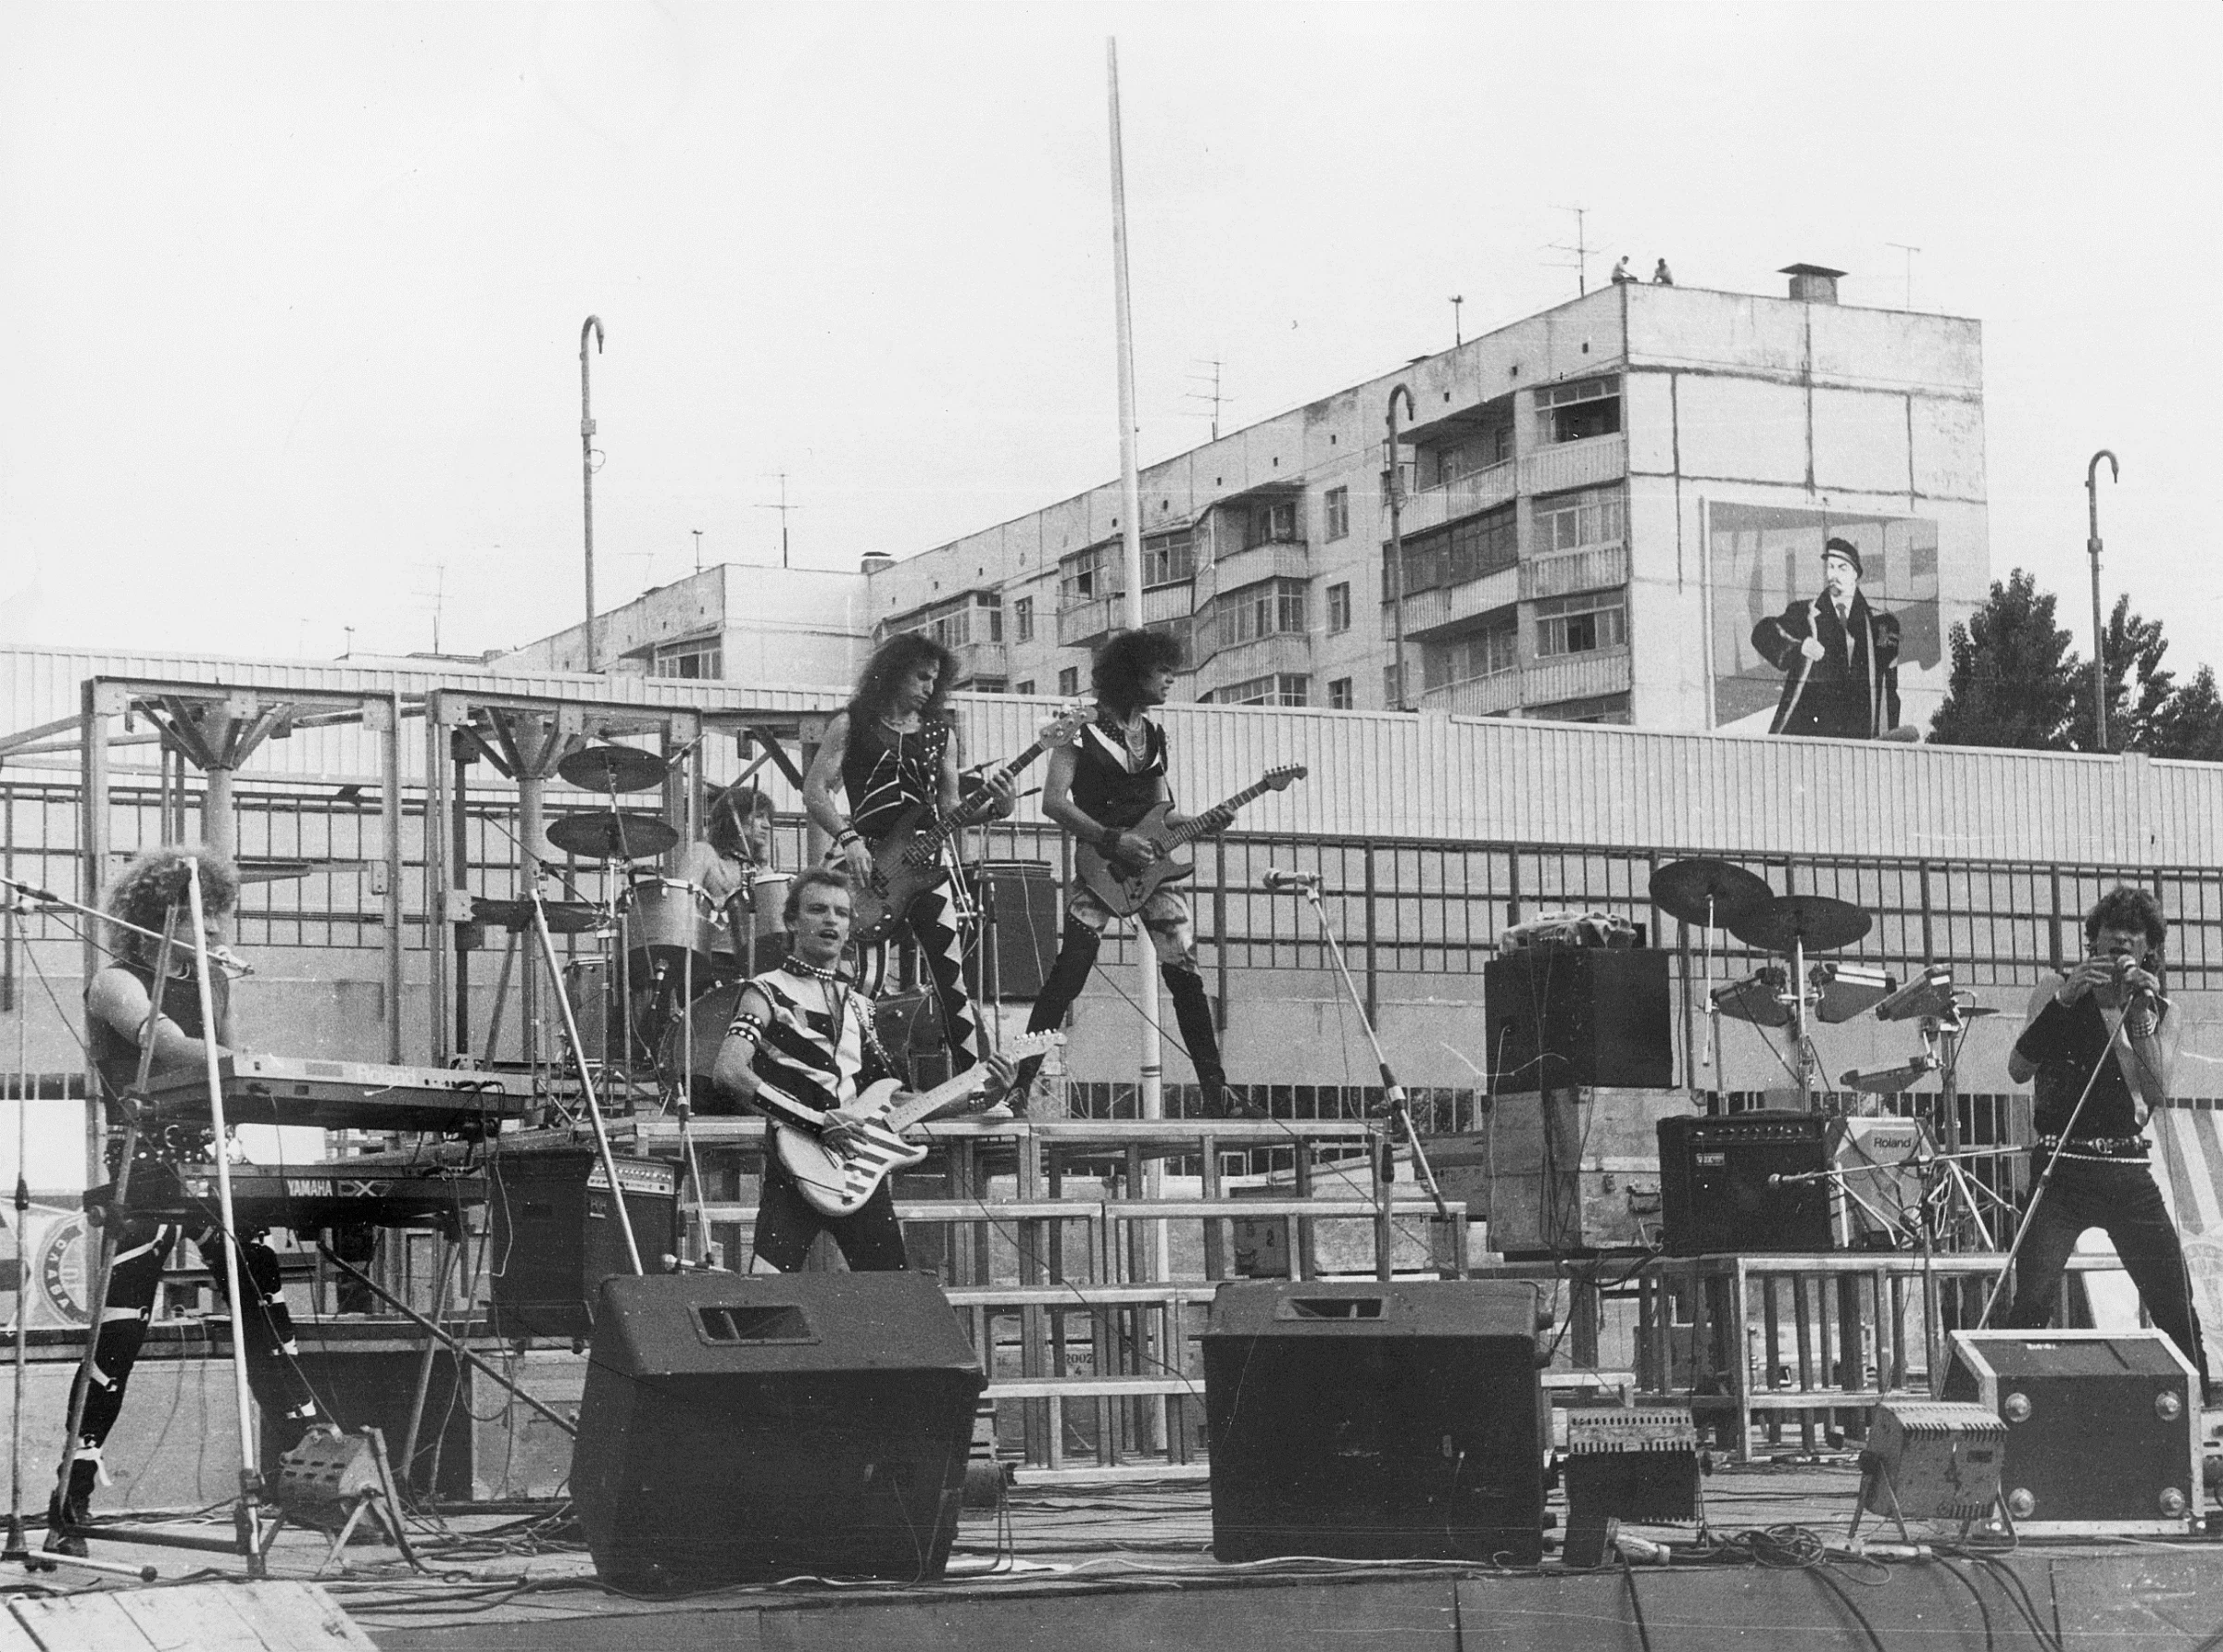
\includegraphics[scale=0.8]{Image19}
    \caption{\textit{Херсон. Концерт с Гошей Корнеевым}}
\end{figure}

Когда группа вернулась с гастролей, Гольденберг вызвал к себе Большакова, исполнявшего обязанности руководителя
коллектива, и устроил ему нагоняй по всей форме: «Срочно ищите вокалиста! Берите кого хотите, но вы обязаны играть,
потому что я из-за вас «палки» терять не намерен!» («Палками» на филармоническом слэнге называли концерты. Проехали
город, в графике одну палку зачеркнули — значит, работа проведена.)

Вот тогда в группе и появился Михаил Серышев. Его привел в «Мастер» Александр Елин, который будучи близким другом
Большакова, вместе со всеми покинул «Арию» и продолжал писать тексты для «Мастера». Елин услышал от знакомых, что в
филармонической группе «Час пик» работает классный вокалист, который одновременно ищет «правильную» команду, поскольку
«Час Пик», похоже, скоро прекратит свое существование.

Серышев пришел на прослушивание: красивый парень с приятной внешностью и длинными волосами, явился в компании с
беременной женой. Михаил идеально повторил партии Кипелова, чисто взяв все ноты с хорошей подачей. У него был такой же
тембр голоса, что и у Кипелова: классический тенор, — по этой причине претендент подходил «Мастеру» по всем параметрам.
Грановский сразу отметил, что наличие у Серышева подобного тембра голоса являлось очень важным для «Мастера», так как
переориентировать группу, то есть начинать писать песни для другого голоса было уже невозможно, да и времени на это не
было.

\begin{wrapfigure}{R}{0.5\textwidth}
    \centering
    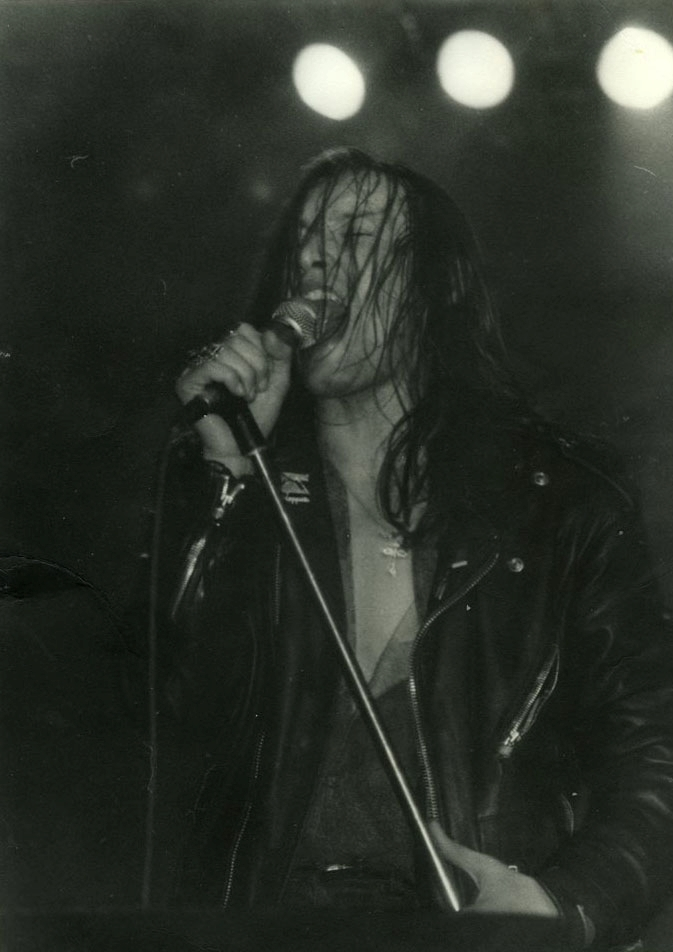
\includegraphics[scale=0.9]{Image20}
    \caption{\textit{Михаил Серышев}}
\end{wrapfigure}

Однако Большаков хотел продолжить поиски — рок-музыка только что вышла из подполья и музыканты хотели проявить себя с
лучшей стороны, так что вполне реально было найти профессионального вокалиста с необычным тембром голоса, но тут в
защиту Серышева выступил Гольденберг: «Я не знаю, как с точки зрения «нравится — не нравится», но он — «рабочий конь», у
него большой опыт гастролей в прежней группе, поэтому пусть он работает».

— Валера, ты же сказал, что не будешь лезть в творчество! — возмутился было Большаков.
— А я не в творчество лезу, — резонно заметил Гольденберг — Это — мои деньги! Я зарядил гастроли — и вы обязаны их
отработать.

Вся вторая половина 1987 года прошла в бесконечных гастролях. И везде нашим героям сопутствовал прямо-таки оглушительный
успех. В итоге те три группы, что выступали в одной программе с «Мастером» — «Браво», «Рондо» и «Зеркало мира» —
Гольденберг отпустил, и «Мастер» теперь работал сольные концерты на стадионах и во Дворцах спорта. И даже на сольных
выступлениях группы всегда был аншлаг.

В Свердловске «Мастер» пробыл две недели, выступая дважды в день и собирая по пять тысяч зрителей на каждый концерт.

В Одессе толпа фанатов устроила жуткий погром в Зеленом театре, где выступал «Мастер», и оставшиеся концерты были
отменены. На следующий день в семь часов вечера все, кто должен был прийти на концерт, отправились к гостинице
«Красная», в которой остановились музыканты, по пути увлекая за собой все новых и новых поклонников «тяжелого металла».
Возбужденная толпа запрудила площадь перед гостиницей, полностью парализовав движение транспорта. В течение пяти часов
над площадью разносились крики «Мастер», а Большаков время от времени выходил на балкон и как Ленин махал рукой, а затем
убегал обратно в номер. Похожая ситуация в той или иной форме повторялась почти в каждом городе. Крайняя популярность
«металлической» музыки была неимоверно усилена буквально витавшей в воздухе свободой освободившейся из-под долгого
социалистического ига страны.

Но концерты концертами, а по правилам шоу-бизнеса каждый успех надо закреплять записью. В начале зимы 1988 года
Гольденберг объявил музыкантам, что пора ехать на «Мелодию» и записывать пластинку. В конце января работа над записью
была окончена, а в начале октября пластинка уже появилась на прилавках магазинов. И хотя об этом не писал «Московский
комсомолец», первый диск «Мастера» стал безусловным лидером продаж года: общий тираж пластинки составил более трех
миллионов экземпляров.

\begin{figure}
    \centering
    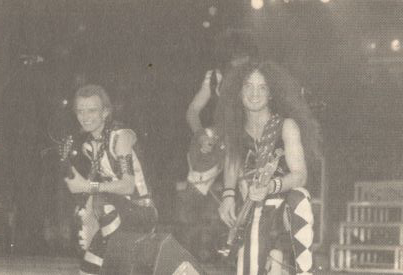
\includegraphics[scale=0.9]{Image21}
    \caption{\textit{1987 год. Концерт в ЦДТ}}
\end{figure}

Векштейн, прослушав пластинку, сказал вслух то, что подумал: «А играют-то они круто!». И тут же обратился к своим
музыкантам: «Ну, а вы-то так сможете?!». Впрочем, им совсем незачем было играть так же быстро и агрессивно, ведь у
«Арии» героическими усилиями Володи Холстинина выработался совершенно иной стиль, который нашел отклик в сердцах
миллионов поклонников по всей стране. Просто у «арийцев» еще не вышла ни одна виниловая пластинка. Но когда Большакову
передали эти слова, нечаянно вырвавшиеся из уст его бывшего шефа, Андрей был доволен: «Мне ничего другого и не надо
было. Нравится музыка или не нравится — это дело вкуса, а тут: «играют-то круто»! Это была наша маленькая победа!».

Массовая популярность «Мастера» была основана на музыке, которую одни называли «красный металл», а другие — «поп-трэш»,
то есть «популярный трэш», в этом динамичном стиле яростные современные ритмы соединены с мелодией. Большую роль играла
зрелищность выступлений, музыканты «Мастера» были одеты в разноцветные костюмы и ярко накрашены. Такова была
принципиальная установка, тот стратегический ход, который дал в итоге необходимый эффект. Сначала музыканты «Мастера» не
хотели использовать косметику, но Большаков, будучи формальным руководителем ансамбля, настоял на этом: «Меня музыканты
спрашивали: зачем это нужно? Но я всякий раз отвечал одно и то же: «Мы будем краситься, потому что сейчас время
краситься!». Пацаны-«металлисты» реагировали на кожу, клепки и «тяжелые» риффы, а девушки на мелодику и веселый
грим\ldots «Нам нужны были и те, и другие, — говорит Большаков. — У меня до сих пор лежат письма, которые нам присылали,
и даже книги, которые про нас писали, неизданные книги о том, какие мы клевые и хорошие. Мы приезжали в какой-то город —
к нам тут же приваливали тучи группис (за рубежом так называют девушек, следующих за любимыми рок-артистами, зачастую
преданных им не только душой, но и телом), они даже еду для нас с собой приносили и кормили нас всякими домашними
разносолами\ldots»

Теперь, когда победа на внутреннем рынке была достигнута, пора было отправляться покорять заграницу — и Гольденберг
устроил «Мастеру» пробную поездку в Польшу. Кроме «Мастера» в десантную группу вошли артисты популярного жанра Михаил
Муромов, Тамара Гвердцители, Владимир Кузьмин и Лариса Долина. Устроена поездка была из рук вон плохо: то аппаратуру
забывали подвезти, то афиши развесить, то еще какие-то накладки случались. А на концерте в Кракове Большаков и вовсе
травму получил. Начиная играть первую вещь, музыканты «Мастера» обычно поднимались на подиум, где стояли барабаны, и все
одновременно спрыгивали с него. Так было и в тот раз, но когда Андрей прыгал, гитара ударилась ему о колено и, отскочив,
попала прямо в бровь. Лицо Андрея тут же залила кровь. Его увели со сцены и попытались оказать первую помощь, но кровь
никак не останавливалась и весь тот концерт «Мастер» отыграл без Большакова.

\begin{figure}
    \centering
    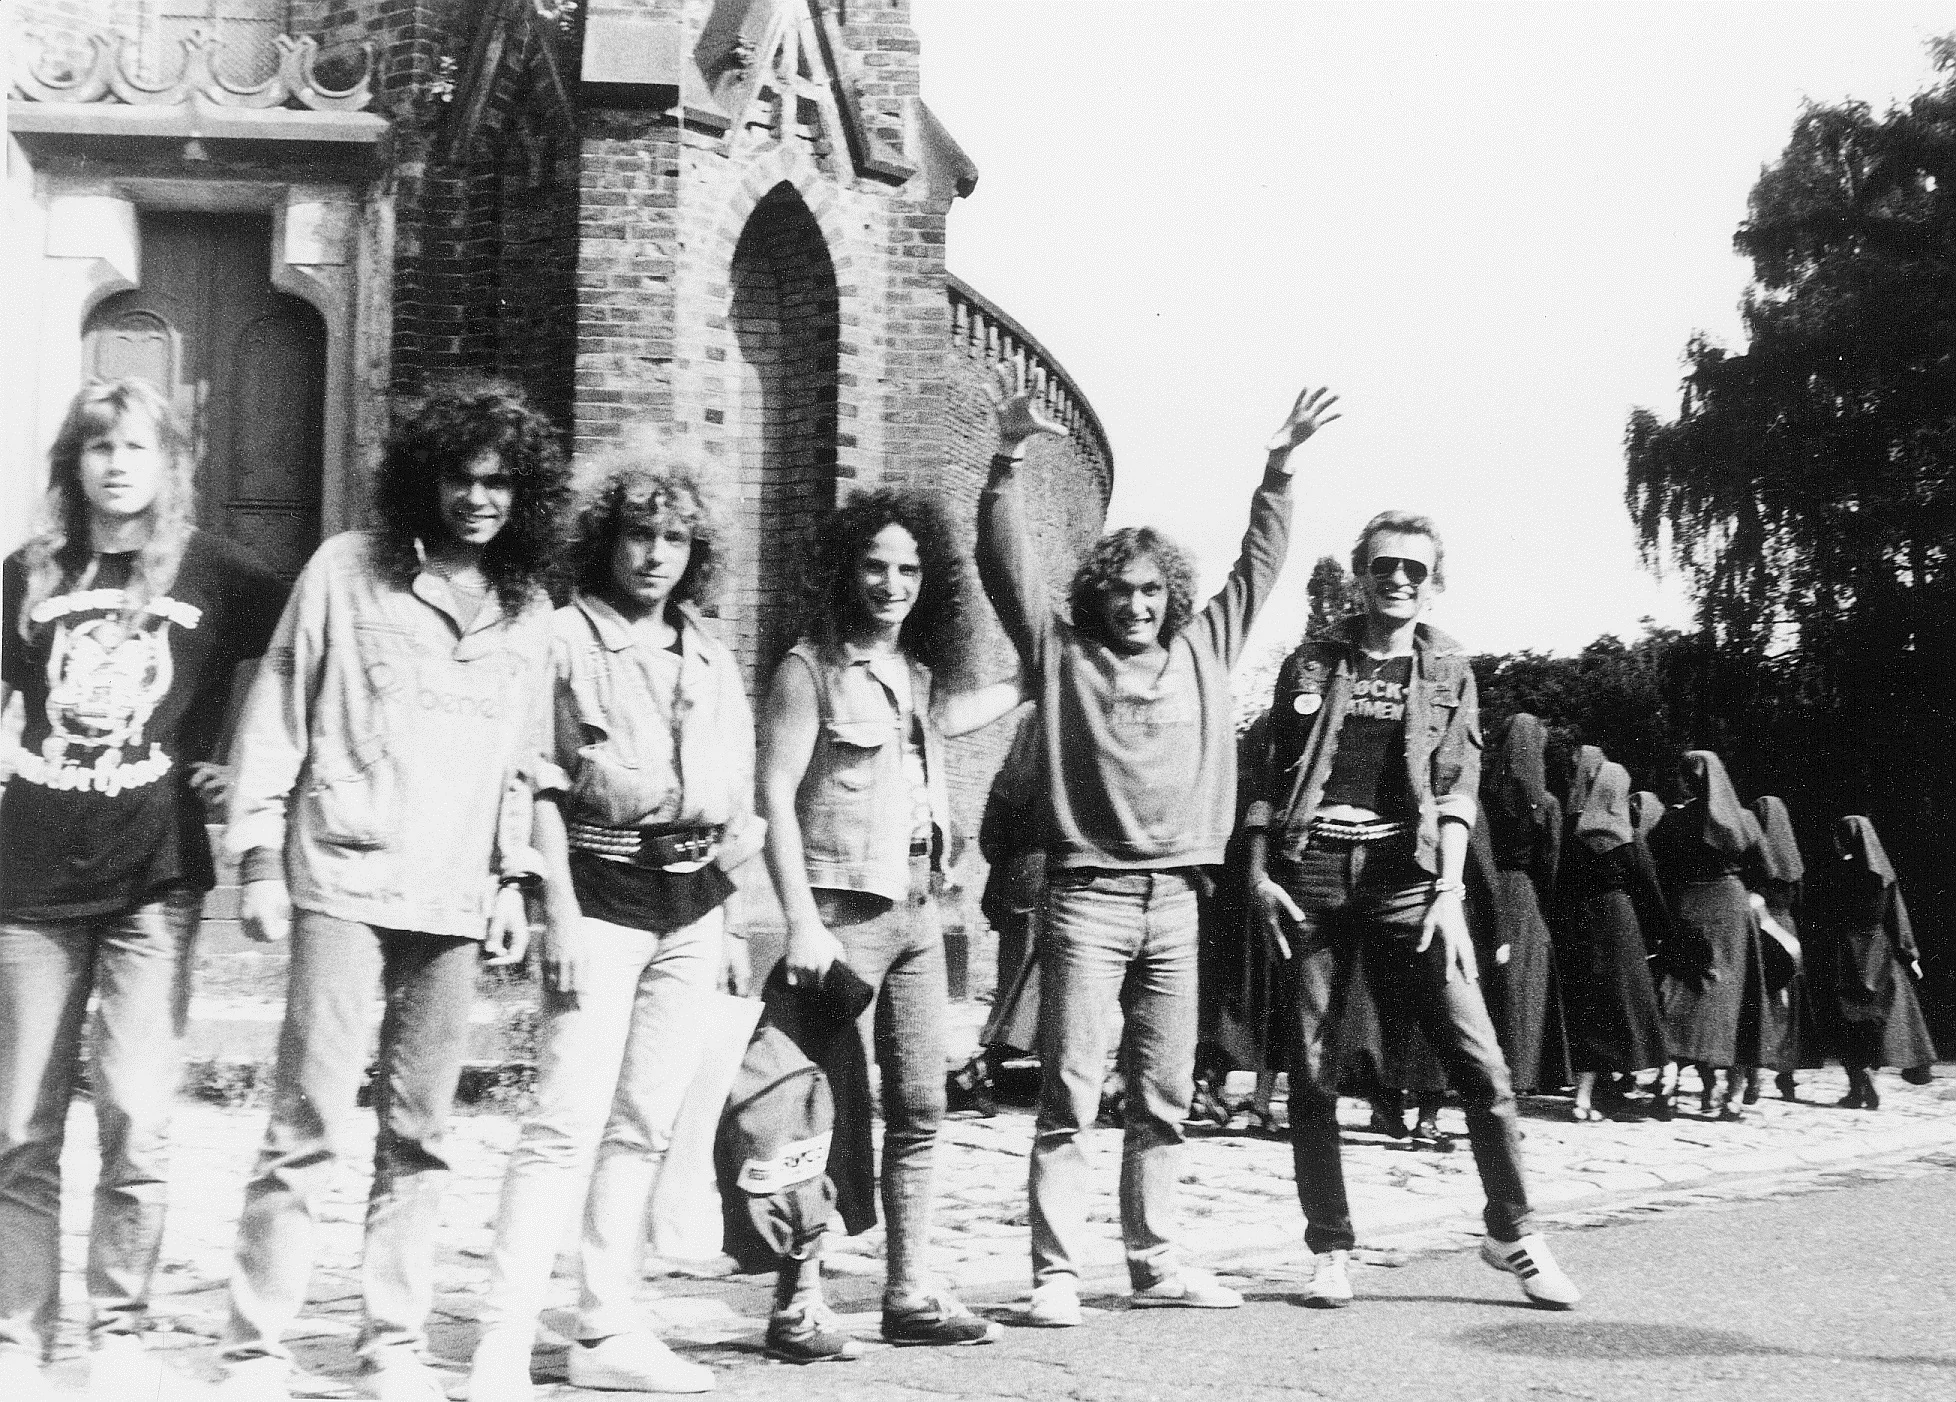
\includegraphics[scale=0.8]{Image22}
    \caption{\textit{«Мастер» в Польше}}
\end{figure}

Нужна ли была такая поездка «Мастеру»? Да, потому что по тогдашним правилам советский человек не мог поехать в
капиталистическую страну, не побывав предварительно в стране из социалистического лагеря, например, в Польше. А после
того как «Мастер» съездил в Польшу, Гольденберг договорился о поездке поездке в Бельгию.

Это тоже была поездка по культурному обмену. К нам, в Советский Союз, из Бельгии приехали какие-то театры, художники и
писатели, а в Бельгию из СССР отправились космонавты, труженики села, народный хор, а также две рок-группы «Динамик»
Владимира Кузьмина и «Мастер».

Концерты «Мастера» вызвали в Бельгии настоящий ажиотаж среди любителей «тяжелой» музыки, потому что никто не ожидал
услышать от русских настоящий «хэви-металл». Когда выступление «Мастера» закончилось, музыкантов тут же окружили
новоявленные бельгийские фанаты. Все знали, что в России есть волки и медведи, но что там встречаются и профессионально
играющие «металлические» команды — такого не могла вообразить самая изощренная западноевропейская фантазия. Поэтому
каждому из пришедших на концерт хотелось дотронуться до удивительных русских, а — если удастся — то и поговорить.

Сквозь плотное кольцо желавших пообщаться с русскими музыкантами пробился известный в Бельгии человек, дизайнер и
фотограф, оформлявший пластинки группы «Хелловин», друг «Айрон Мэйден» и «Металлики» Фредерик Мулар: «Хэлло, бойз, —
сказал он, — мне очень понравилась ваша группа, и вообще это очень необычно видеть здесь группу из России. Здорово, мне
понравилось! Я многих знаю, многих видел, но у вас есть что-то свое. Только очень уж у вас непонятный и смешной язык».

Слово за словом, кружечка бельгийского пива за стаканчиком шотландского виски — и компания постепенно переместилась в
дом гостеприимного Фредерика. А когда музыканты уходили, он спросил:

— А почему бы вам не приехать сюда еще раз?
— Это было бы здорово, но как это сделать?
— Да очень просто: я вам приглашение вышлю\ldots

Через несколько месяцев вызов действительно пришел.

\begin{wrapfigure}{R}{0.5\textwidth}
    \centering
    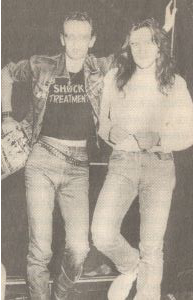
\includegraphics[scale=0.9]{Image23}
    \caption{\textit{Андрей Большаков и Фредерик Мулар}}
\end{wrapfigure}

Во вторую поездку у «Мастера» было запланировано два концерта в брюссельских клубах. Когда «Мастер» отыграл второй
сейшен, группу в качестве special guests (специальных гостей) пригласили на фестиваль бельгийских команд, проходивший в
Брюсселе. Присутствовало огромное количество зрителей, так как в программе значились лучшие бельгийские «тяжелые»
группы. Наши герои поначалу тушевались, жались к стенкам, но потом вслушались в то, что звучало на сцене. Все группы
играли профессионально, но они были явно вторичны: одни работали под «King Diamond», другие — под «Def Leppard», ничего
своего, кроме разве что французского языка. К тому же все бельгийские группы выглядели очень статично, музыканты были
будто привязаны к своему месту на сцене, словно они играли не рок-музыку, а скрипичные концерты. На этом фоне
выступление «Мастера» выглядело как настоящее рок-н-рольное шоу, эдакая смесь хорошей музыки и полной сценической
раскрепощенности.

В таком сценическом напоре и натиске суть успеха «Мастера» в Бельгии. Ведь Бельгия – это очень спокойная, комфортная и
удобная для жизни страна, поэтому даже «металлические» команды там играют очень правильно, стандартно и абсолютно без
фантазии. И тут появляются эти безбашенные русские и рубятся на сцене так, словно это — то ли их последний в жизни
концерт, то ли звездные войны\ldots Бельгийские поклонники «тяжмета» не могли не оценить этот прорыв в Запределье. Все
они были наслушанными в тяжелой музыке людьми, впрочем, и дилетанту было понятно, что выступала действительно хорошая
группа.

Сыграл свою роль и сценический имидж «Мастера». Поскольку все музыканты были причудливо раскрашены, на выступление
пришло большое количество падкой на внешний эффект публики, в первую очередь — бельгийских девченок, которые и создавали
основную бурлящую вокруг нашей группы массу.

\begin{figure}
    \centering
    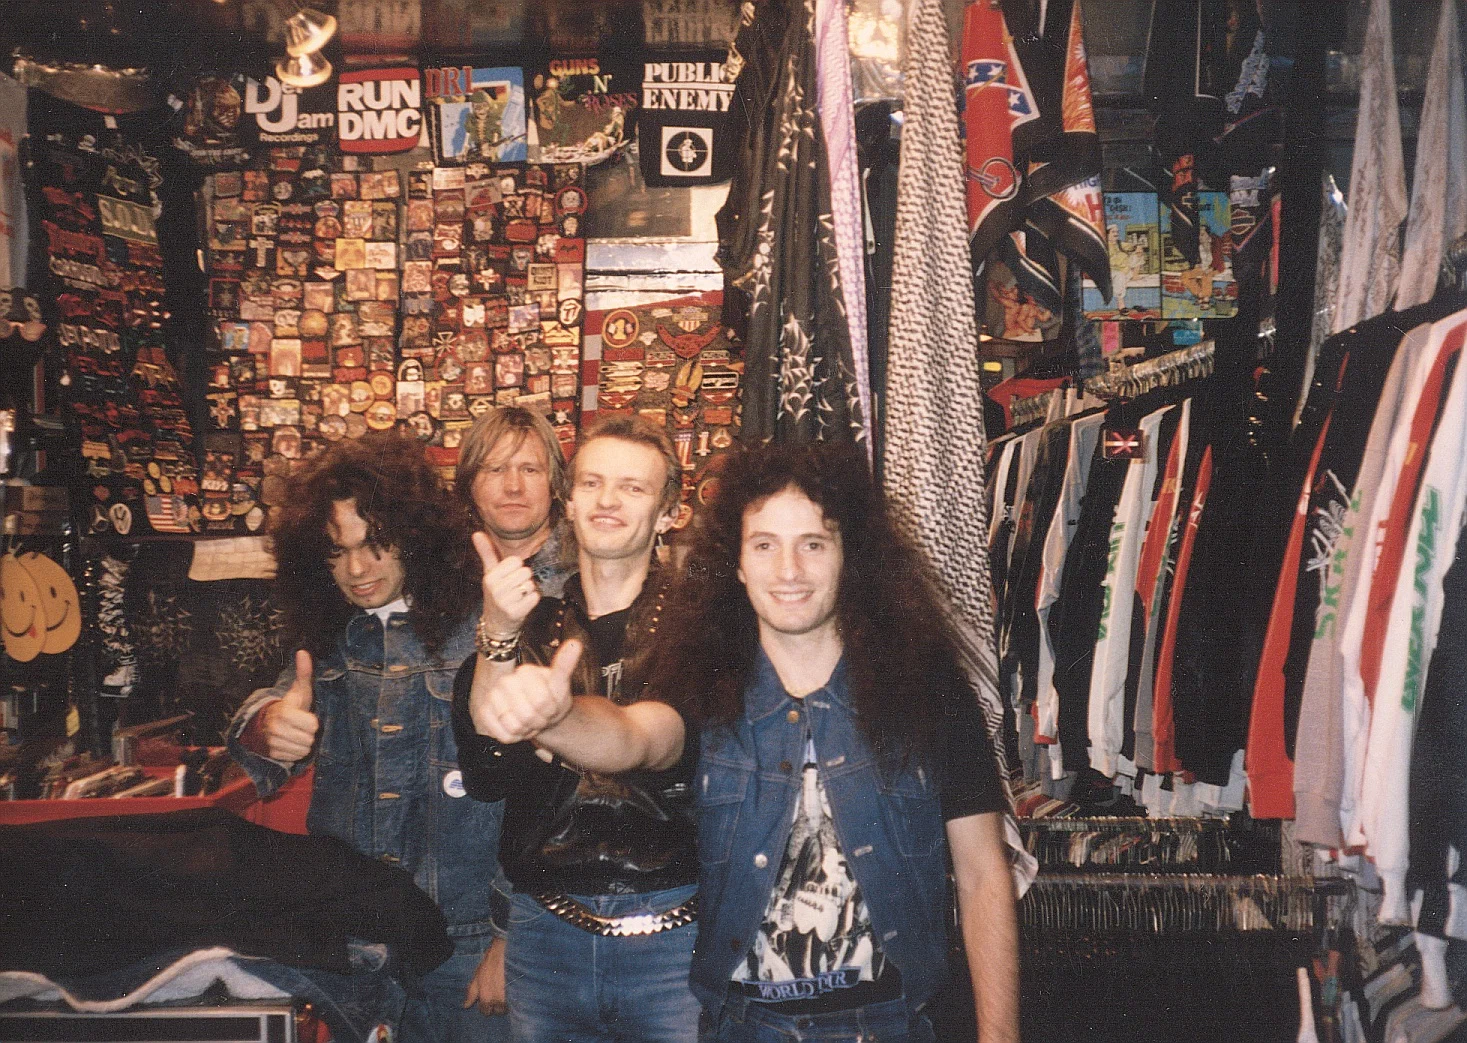
\includegraphics[scale=0.8]{Image24}
    \caption{\textit{«Мастер» в самом крутом металлическом магазине Бельгии}}
\end{figure}

Не надо также забывать, что группа исполняла абсолютно накатанную и до блеска отшлифованную программу, ведь на пике
своего успеха «Мастер» давал по 50-60 концертов в месяц. Конечно, музыканты уставали, и однажды приехав офис к
Гольденбергу Большаков взмолился: «Валера, ну сколько можно пахать! Ведь мы работаем по четыре концерта в день! Мы
устали. Мы хотим отдохнуть». На что Гольденберг загадочно ответил: «Потерпите немножечко, и вы отдохнете. И отдыхать
будете долго!». Сначала Большаков подумал, что их продюсер шутит, но потом музыканты узнали, что Гольденберг взял под
опеку становившийся популярным «Ласковый май». В то время это был один из наиболее кассовых проектов, и Гольденберг
просто переключился на него, забыл о существовании «Мастера», Тогда Большаков снова поехал к нему и с порога объявил:

— Валера, учитывая, что количество концертов резко уменьшилось, а мы с тобой договаривались, что концертов будет много,
мы от тебя уходим!
— Что!!! Вы от меня уходите?! Нет, это я от вас ухожу! — напрягся Гольденберг.
— Хорошо, ты можешь считать по-своему, а мы будем считать именно так, — сказал Андрей, повернулся и вышел.

После этого Большаков с Молчановым поехали на свою репетиционную базу в «Крылья Советов», где как раз шел концерт
«Ласкового Мая». В зале биток народу! Музыканты остановились в проходе, бабушки-контролерши узнали наших героев и сразу
запричитали: «Господи, ужас-то какой! Эти-то в тренировочных выступают, будто сироты казанские! То ли дело было на ваших
концертах: все аккуратненькие, в курточках на молниях\ldots».

Тут как раз из служебного входа появился Гольденберг.

— Валера, мы приехали вещи наши забрать\ldots
— Да забирайте!.. — бросил он небрежно, но вдруг остановился и сделал рукой широкий жест сторону беснующегося под «Белые
розы» (суперхит «Ласкового Мая») зрительного зала, — Вот смотрите, как надо работать!
— Валера, да ты вспомни, как совсем недавно тут работали мы, и у нас было десять аншлагов. А у этих только один
аншлаг!..
— Да так было, но ваше время ушло\ldots
— Валера, но ты же предал нас и нашу музыку!
— Извините, ребята, ничего личного — только бизнес\ldots — ответил Гольденберг и, махнув на прощанье рукой, ушел по
своим делам.

Шел 1989 год. «Перестройка» фактически закончилась, окончился и небывалый расцвет музыки «хэви-металл», крайне популярны
стали многочисленные «Миражи» да «Ласковые маи»\ldots А «Мастер» через некоторое время снова уехал в Бельгию\ldots

Гольденберг исчез за горизонтом, зато из Карельской филармонии в Москву вернулся Андрей Крустер. Он давно уже наблюдал
за успехами друга, а однажды они встретились на гастролях. Крустер в то время работал администратором у Андрея Рублева,
бывшего вокалиста питерской хард-роковой группы «Август». Как-то он отправился договариваться о концертах в город
Кировоград, где в это время гастролировал «Мастер». Андрей пришел на концерт, а вечером, на торжественном ужине, было
решено, что Крустер переходит на работу в «Мастер». В тот момент из группы уходил звукорежиссер Юрий Соколов, который
решил собрать свой собственный комплект звуковой аппаратуры и заняться организацией концертов (сегодня Юрий Соколов —
продюсер группы «Ария»). Но так как он был одним из лучших звукорежиссеров в стране, то заменить его за пультом было не
просто. Именно Крустер являлся одним из немногих, чья квалификация позволяла сделать это. Но Крустер пришел не один, а
со своим соратником по «Млечному Пути» Михаилом Павловым, у которого в свою очередь был друг Леонид Ненашев, сын певицы
Галины Ненашевой, а та являлась владелицей «фирменного» комплекта аппаратуры фирмы «Реаvеу» и собственной базы. И эта
аппаратура, и эта база в ДК «Высотник», расположенного в Раменках, оказались в полном распоряжении группы «Мастер».

Крустер и Павлов немедленно организовали концерт в ДК МИСИ, прошедший с аншлагом, а затем группа выехала в тур — все
снова пошло своим чередом.

Во время гастролей создавались новые песни, из которых постепенно складывалась новая программа. Грановский и Большаков
запирались в номере (если были на гастролях) или на репетиционной базе, где отрабатывали и совершенствовали домашние
заготовки — гитарные риффы новых песен. Грановский написал песню «Иуда». Большаков сочинил композиции «Не хотим»,
«Палачи», «С петлей на шее», «Когда я умру», «Мы не рабы» и «Наплевать!». Две шикарные вещи принес Попов — «Боже, храни
нашу злость» и «Война». Внес свою лепту в общее дело и Кирилл Покровский, написавший «Семь кругов ада».

Это было время творческого подъема, когда в группе творили все. При этом музыка «Мастера» была достаточно необычна для
того времени. С начала 80-х годов на территории страны доминировала ленинградская школа рока, по сути — бард-рок, в
котором стихи рождаются раньше мелодии или одновременно с ней. Поскольку любой стихотворный размер уже диктовал свои
требования музыкальному обрамлению, музыка становилась вторичной. Группа «Мастер» шла иным путем. Сначала появлялась
мелодия, ритмика, аранжировка, а только потом на фактически готовую музыку поэты писали тексты. Подобный подход ставил
во главу угла именно рок-музыку, после чего оставалось крайне важное дело — написать идеально подходящий для музыки
текст, что было под силу только профессионалам высокого класса.

Но насколько такой подход органичен для рока? Не должен ли человек сам писать слова, раз он их поет? Поэт Александр Елин
говорит об этом так: «Мы настолько давно были знакомы с Большаковым, у нас были настолько схожие музыкальные
пристрастия, общие книги, которые мы читали, общие темы разговоров, что меня можно вообще не рассматривать как человека,
который писал тексты для группы «Мастер», — мною, как ручкой, водил Большаков. Я приносил какие-то слова, но потом все
равно Большаков сидел и доводил их до ума. И так происходит всегда, когда поэт правильный. Тогда он уподобляется некоей
ручке для музыканта, который продюсирует музыку, потому что все равно последнее слово за ним\ldots».

Однако поскольку Александр Елин был в это время занят собственным проектом «Примадонна», Большаков призвал под знамена
«Мастера» двух поэтесс — Маргариту Пушкину и Нину Кокореву.

С Ритой Пушкиной Андрей познакомился еще во времена работы в «Арии», именно она написала тексты двух ранних «арийских»
хитов — «Тореро» и «Без тебя». Когда пришла пора делать новую программу, Большаков позвонил Рите и предложил
сотрудничество. Он передал Пушкиной демо-кассету с записанной музыкой, она выбрала две композиции и написала тексты
«Боже, храни нашу злость» и «Мы не рабы».

Нина Кокорева работала вместе с Ладой, женой Большакова. Узнав однажды, что муж Лады — музыкант, Нина решилась показать
ей свои стихи, разумеется, сказав при этом, что это творчество ее приятеля. Лада стихи прочла, они ей понравились, после
чего она без обиняков спросила Нину: «Это ты сама написала?..» Тем же вечером Андрей позвонил ей, Нина подъехала к
«Мастеру» на репетиционную базу в кинотеатр «Энтузиаст», и Андрей предложил ей написать текст для песни, которая вскоре
получила название «Берегись». Это была первая песня, написанная Кокоревой для группы «Мастер». Если для первой программы
она сочинила лишь один текст, то для второй написала уже четыре песни: «Не хотим», «Палачи», «Наплевать!» и «С петлей на
шее».

Новые песни уже звучали на концертах. Но сами музыканты понимали, что для закрепления успеха нужно срочно выпускать
вторую пластинку. С «Мелодией» удалось договориться на удивление легко, впрочем, там прекрасно помнили, как хорошо
продавалась первая пластинка «Мастера». Летом 1989 года альбом был записан и уже зимой появился на прилавках магазинов.
Правда песня «С петлей на шее», давшая название всему альбому, на виниле не вышла. Редакторы фирмы грамзаписи «Мелодия»
во фразе «Миша — это лучшее из имен» усмотрели издевку над Горбачевым. (Полностью этот альбом дошел до глушителей лишь в
1996 году на компактах-дисках фирмы «Мороз Рекордз».)

Повышалось настроение музыкантов в процессе регулярных гастрольных поездок в Бельгию, где местные «металлические»
команды стояли в символической очереди, чтобы сыграть «на разогреве» у «Мастера». Во время одной из поездок наши герои
познакомились с парнем, который работал техником с «Pink Floyd» и «AC/DC», а теперь жил на пособие. Звали его Паскаль
Жуази, и он предложил заняться организацией выступлений «Мастера» в Бельгии.

Так у группы появился за границей свой тур-менеджер, который договаривался об организации концертов и, когда был готов
тур, звонил в Москву и приглашал музыкантов на гастроли. За 1990-91 год «Мастер» побывал в Бельгии (а также в Голландии,
Франции и Люксембурге) девять раз. Поездки обычно длились от двух недель до двух месяцев.

В конце 1989 года во Франции вышел альбом «Destroyka», где среди других хитов русских металлических ансамблей
красовались две песни «Мастера». Этот альбом существенно поднял статус группы среди бельгийских любителей «хэви-металл».

\begin{wrapfigure}{L}{0.5\textwidth}
    \centering
    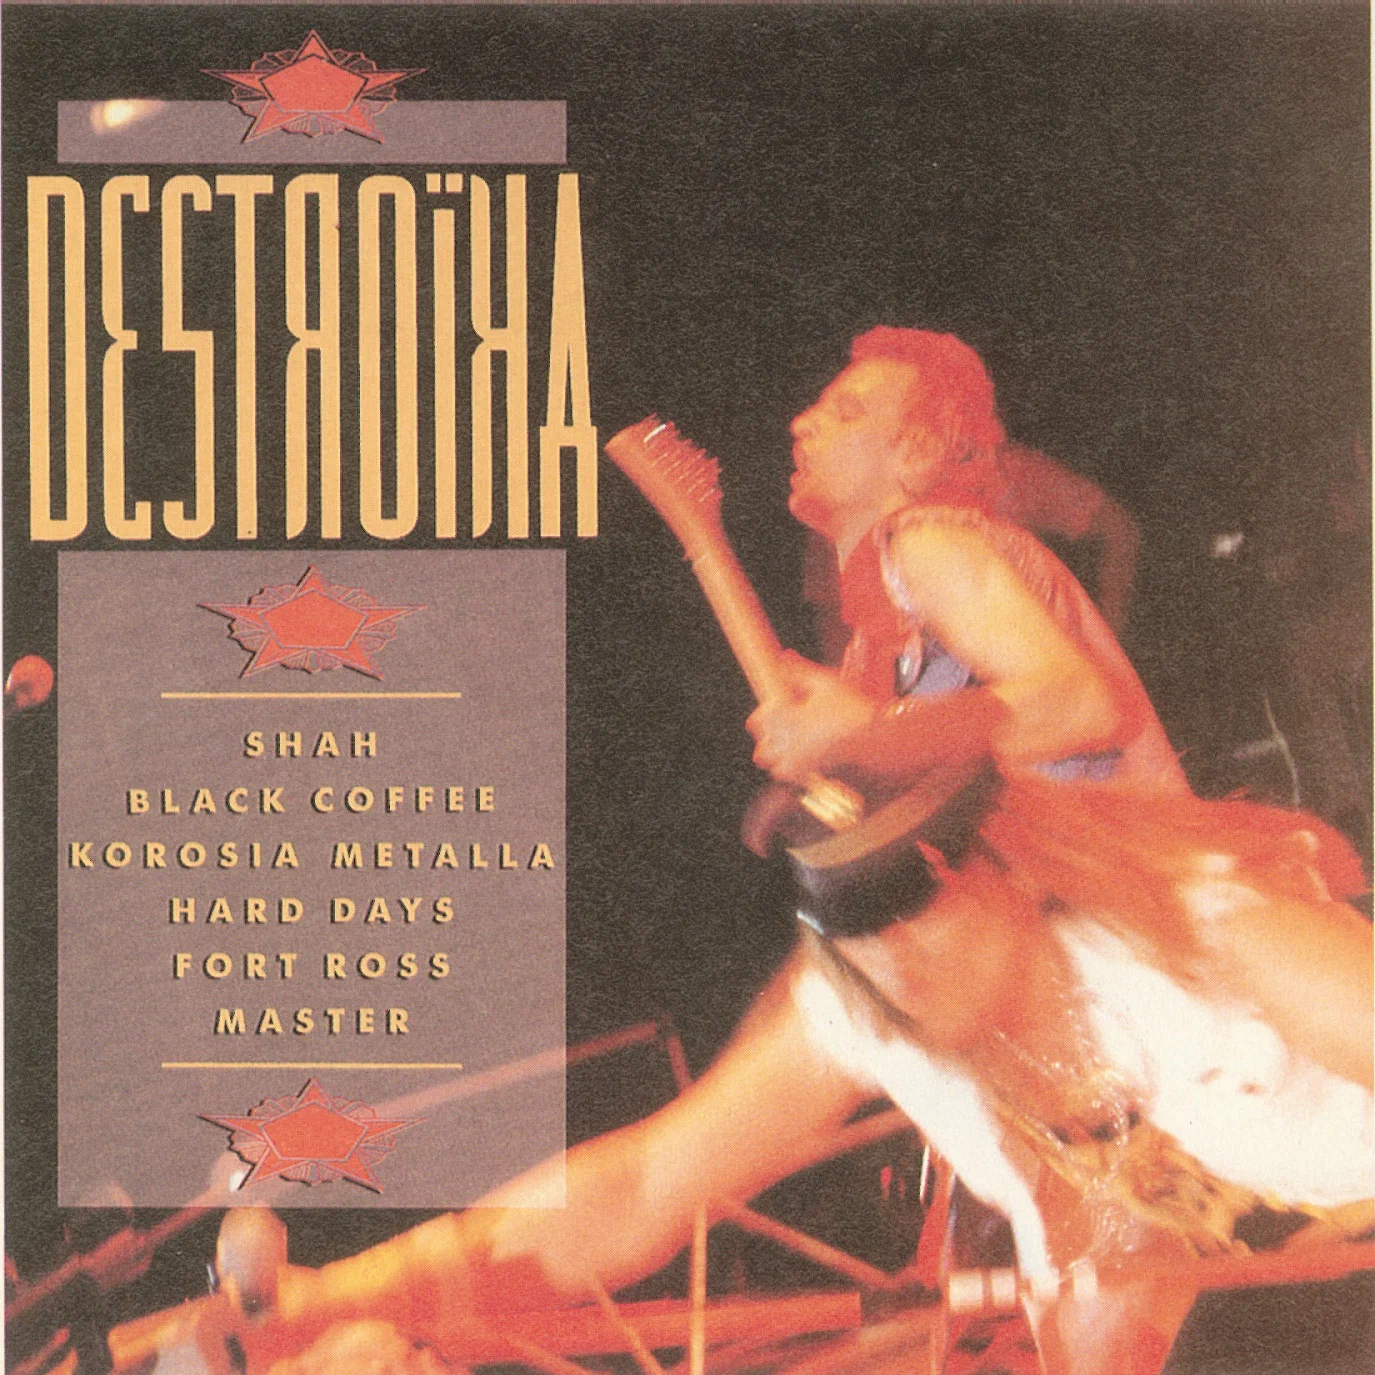
\includegraphics[scale=0.7]{Image25}
    \caption{\textit{На обложке альбома «Destroykа» изображена группа «Мастер»}}
\end{wrapfigure}

Параллельно, по тем же самым бельгийским клубам, что и «Мастер», гастролировала никому еще неизвестная группа «Nirvana»,
но она имела гораздо меньшую популярность среди бельгийских любителей рока, нежели «Мастер», а бельгийские журналисты
откровенно писали, что не понимают, за чем и для кого играется подобная музыка.

К сожалению, с увеличением количества заграничных гастролей у «Мастера» существенно сократилось число концертов на
родине. Зато на первый фестиваль «Монстры рока» в Череповец «Мастер» приехал в статусе «фирменной» команды: буквально
«вечерней лошадью из Брюсселя».

Вообще, российские поклонники группы довольно долго были вынуждены довольствоваться не музыкой, а слухами. И однажды на
российских рок-н-ролльных просторах прошелестела нервная молва о том, что группа «Мастер» распалась. Впрочем, как вскоре
выяснилось, сама группа была цела, невредима и полна творческих планов, просто после одной из бельгийских поездок
коллектив покинул Кирилл Покровский. Еще во время первой поездки в Бельгию он познакомился со звукорежиссером,
пригласившим его работать на своей студии. Покровский был уже не нужен «Мастеру», поэтому он принял это предложение.
Если раньше Грановский и Большаков старались ориентироваться на музыку групп «Rush», «Saga», «Yes» и стремились, чтобы в
их собственных композициях присутствовали клавиши, то теперь «Мастер» начал играть музыку, в которой клавиши бу ли
абсолютно неприменимы, поэтому Кирилл в конце концов решился на то, чтобы кардинально изменить жизнь и остаться в
Бельгии.

Бельгия и Европа сыграли как положительную, так и отрицательную роль в судьбе «Мастера». Положительная заключается в
том, что музыканты сразу же начали по-другому относиться к музыке, ведь они играли с «фирменными» командами и нужно
соответствовать их уровню, для чего пришлось мобилизовать все имеющиеся силы. С другой стороны, западное
рок-пространство трансформировало наших героев под себя. От них требовалось, чтобы программа была сделана совершенно
определенным образом, чтобы Серышев не пел, а рычал, как это принято в каноническом «трэше». Нашелся продюсер, пообещал
выпустить пластинку «Мастера», но его главным условием было, чтобы русская группа пела по-английски. В итоге «Мастер»
сделал шаги к более жесткой, быстрой и агрессивной музыке. Специально для заграницы была сделана типичная программа в
жанре «трэш-металл», а поэт Олег Горбунов написал тексты песен на английском языке. Кроме того музыканты перестали
краситься и переоблачились из разноцветных костюмов в обычные рваные джинсы. Премьера новой программы с названием «Talk
Of The Devil» в Бельгии прошла очень хорошо, поскольку подобная музыка там была весьма модной. Правда, резко изменилась
публика: куда-то исчезли девочки, а их места заняли суровые молодые люди, затянутые в кожу.

\begin{figure}
    \centering
    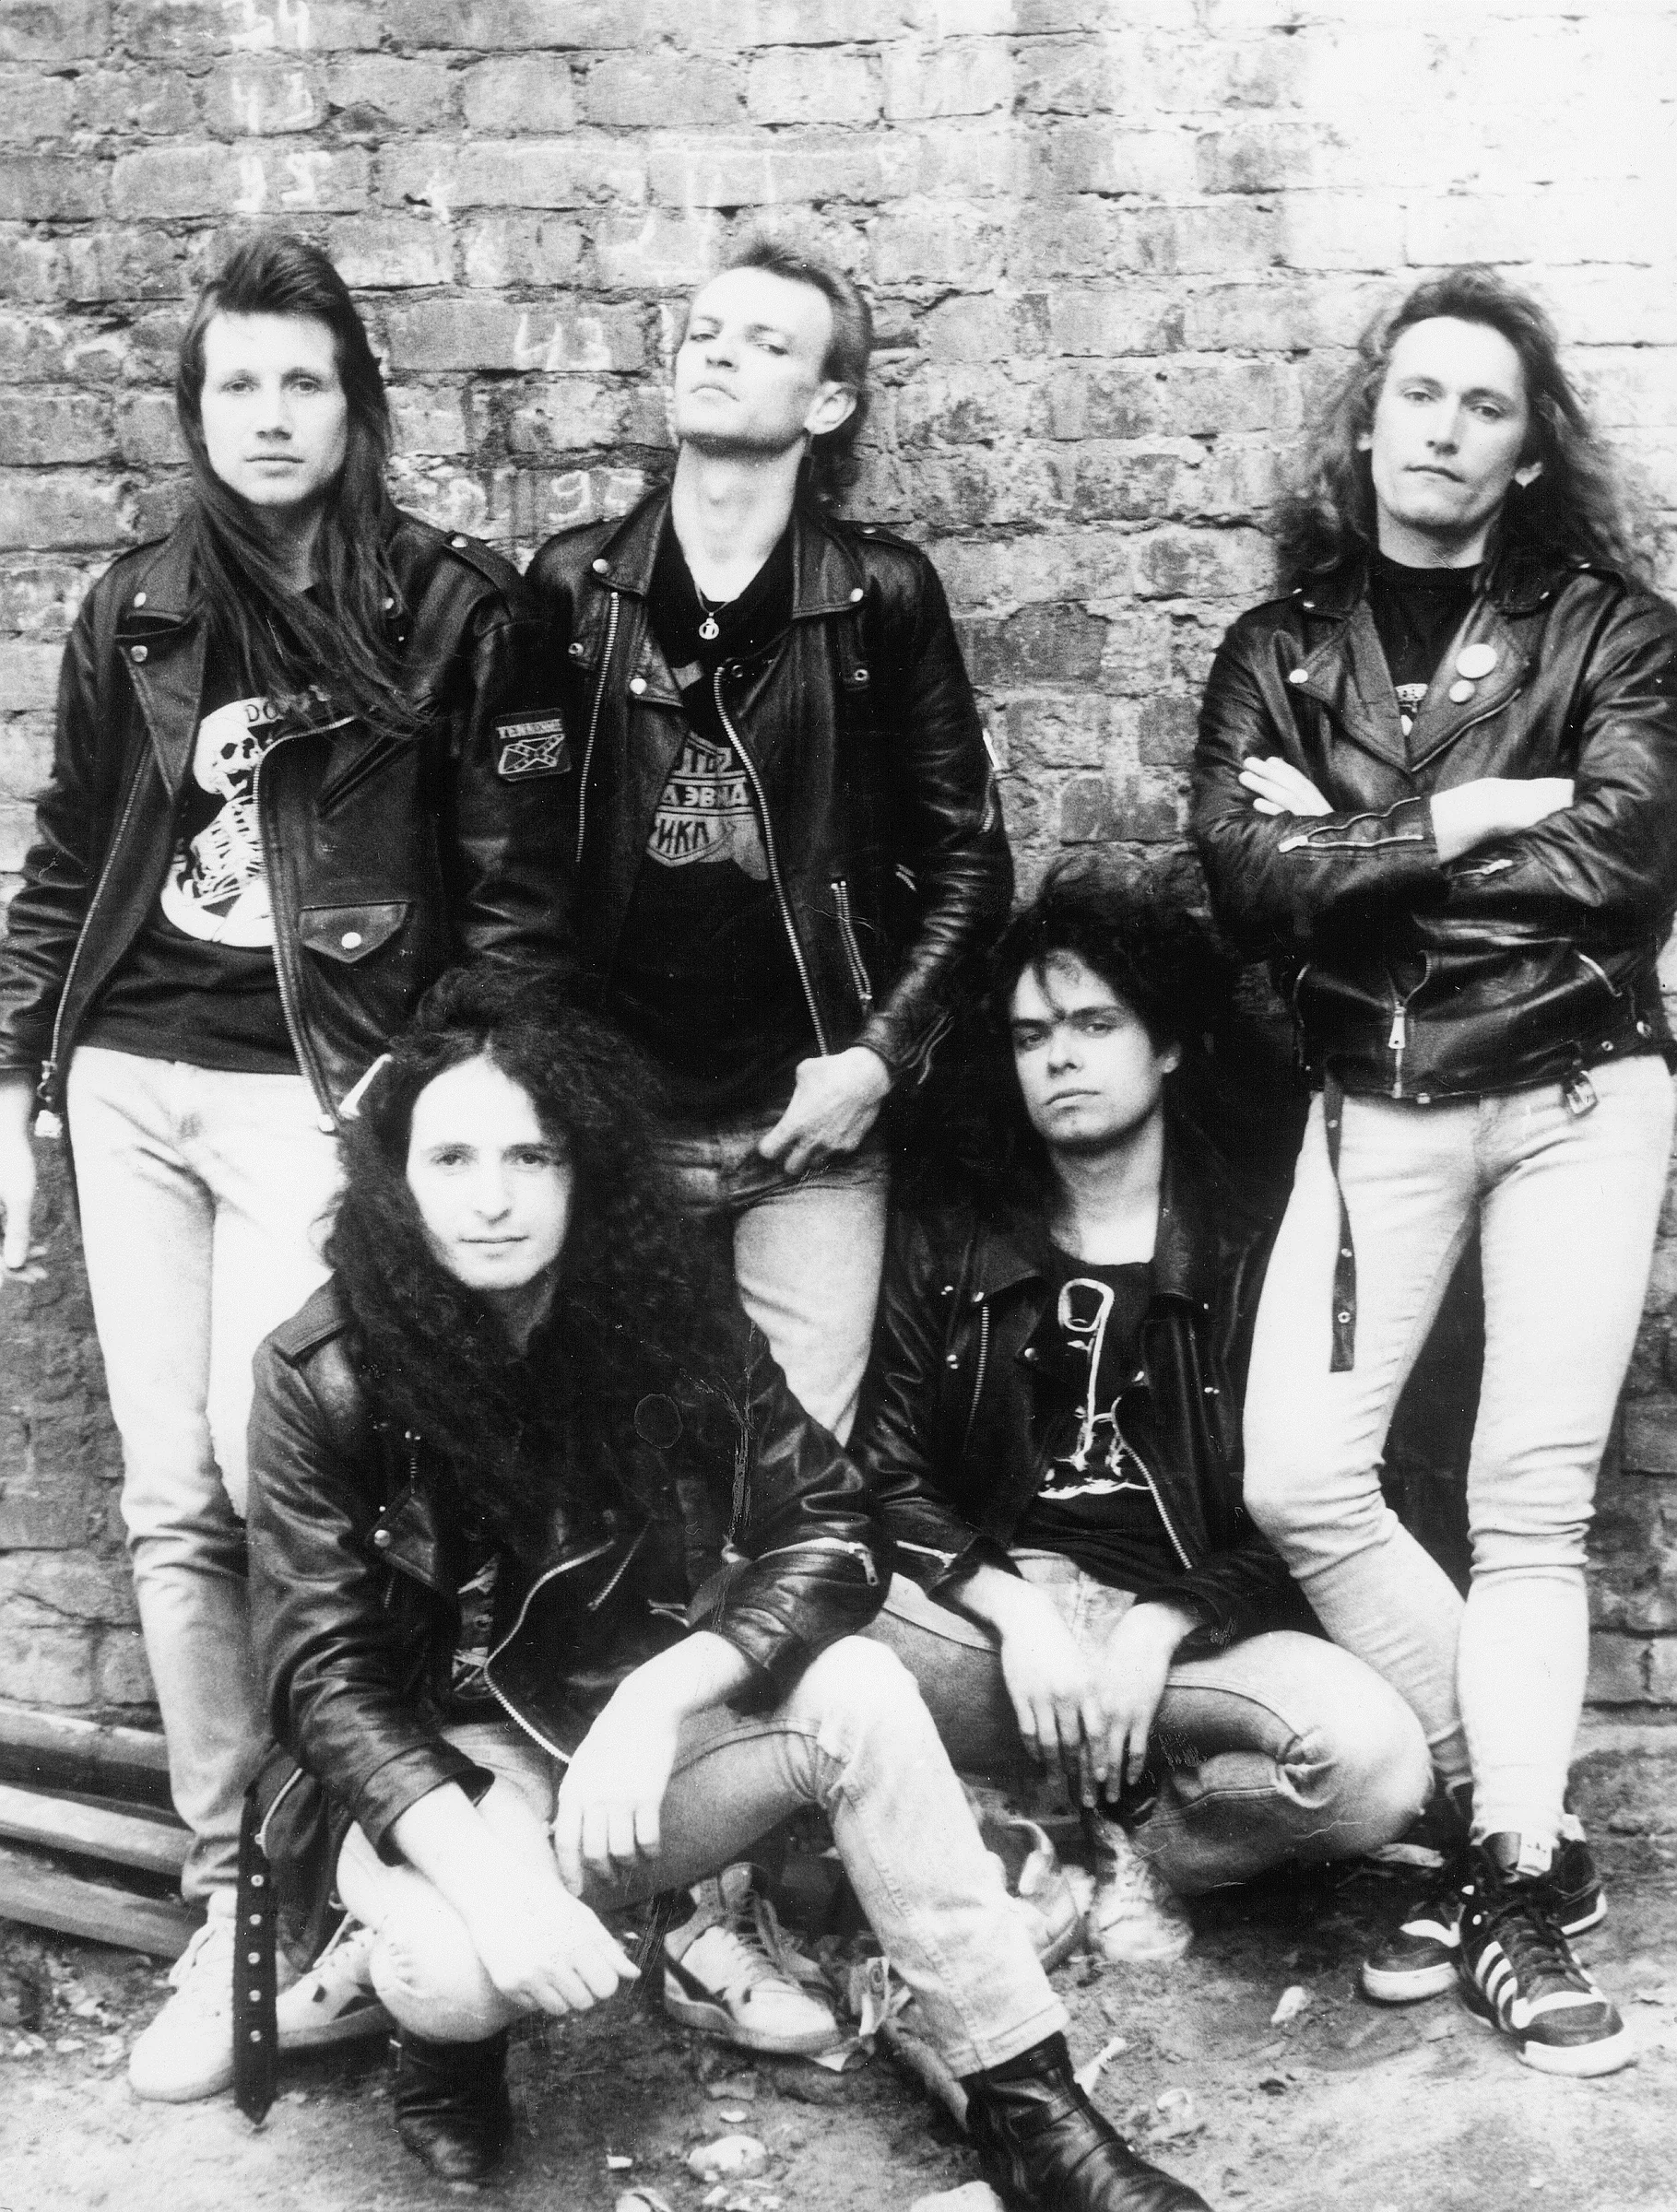
\includegraphics[scale=0.9]{Image26}
    \caption{\textit{В Бельгии музыканты «Мастера» переоделись в джинсы и «косухи»}}
\end{figure}

Фредерик прослушал англоязычную программу и ему не понравилось:

— Ребята, вам надо петь на русском, а так вы потеряли всю свою оригинальность. Вы теперь стали как одна из наших команд.
— Да? Но мы уже договорились выпустить пластинку на английском языке, — ответил за всех Андрей.
— Если так, записывайтесь на английском, — согласился Фредерик. Он конечно понимал, как важно «Мастеру» для дальнейшей
раскрутки выпустить пластинку в Бельгии, но здесь это возможно было сделать только на английском языке.

Переход на английский язык группа приняла отчасти вынужденно. И когда это нелегкое решение было принято, продюсер,
обещавший выпустить пластинку, начал нарушать договоренности. В итоге и подготовленные концерты, и запись отменились.

Паскаль Жуази и Андрей Большаков принялись лихорадочно рыскать по Бельгии и окрестностям в поисках концертов и контракта
на запись и выпуск альбома. И человек, готовый выпустить пластинку «Мастера», в конце концов был найден. Его звали Брюс
Депасс. Он руководил фирмой, которая называлась «Two Flags». Молодой, холеный и очень вежливый, словом, настоящий
бизнесмен. На руках Брюс носил золотые персти, а курил он тонкие черные сигары. Андрей с Паскалем приехали к нему в
офис.

— Да! Я готов за все платить! — сказал Брюс. — Нет проблем! Работаем! Но вам нужно будет остаться еще на месяц, чтобы
записать альбом.
— Ладно, — сказал Андрей. — 0-кей!

А ведь уже месяц прошел, как «Мастер» находился в Бельгии. Причем, наши музыканты успели отыграть только один концерт,
остальные из-за ссоры с продюсером были отменены. Паскаль, конечно, договорился о новых концертах, но их надо было еще
дождаться, а пока музыканты сидели фактически без дела. Целыми днями они играли в компьютерные игры, вечерами, когда их
друзья возвращались с работы, все вместе шли в бар, по выходным отправлялись в путешествие в другие города или к морю.
Такой образ жизни нашим героям быстро надоел, их обуяла смертельная скука, но так как они приехали в Бельгию не на
увеселительную прогулку, а на заработки, то вернуться домой с пустыми карманами они не могли. В итоге скука превратилась
в усталость, что не улучшило взаимоотношений в группе. Когда Большаков сообщил, что придется оставаться еще на месяц,
это никого не обрадовало. Но в конце концов решили, что запись того стоит.

Это была хорошая западная студия, конечно не самая лучшая, но все равно совсем иного уровня, чем на «Мелодии», где до
этого записывался «Мастер». Звукооператора звали Андрэ Гиллан, это был хороший специалист, специализировавшийся именно
на «тяжелой» музыке. Он все предусмотрел, даже наличие в студии человека, который проверял, как Серышев поет
по-английски. И за три-четыре дня, что оставались до отъезда, музыканты «Мастера» записали альбом, после чего собрались
и уехали, оставив Большакова дожидаться подписания контракта.

Каждый день Большаков с Паскалем звонили Брюсу, но тот всякий раз отвечал, что контракт еще не готов, но завтра он его
обязательно пришлет. Так они прождали несколько дней, а срок действия визы у Большакова тем временем подошел к концу.
Наконец он позвонил Брюсу и сказал ему, что контракт ему нужен завтра, потому что послезавтра он должен улететь в
Москву.

— Нет проблем! — отвечает Брюс. — Завтра контракт обязательно будет. Ждите!

Наступило завтра, но никто не привез от Брюса контракта, не отвечал и его телефон. Большаков с Паскалем прождали весь
день, изредка позванивая в офис Брюса, но там, похоже, никого не было, даже секретарши. Андрей нервно ходил по комнате:

— Паскаль, мне сейчас обязательно нужно, чтобы здесь вышел альбом. Ты понимаешь, как это важно?

Потом Большаков начинал мечтать:

— Паскаль, как только выходит альбом, ты нам здесь должен устроить тур для его раскрутки\ldots
— Я всегда готов! — отвечал верный Паскаль.

Андрей снова и снова набирал номер Брюса, но в трубке по прежнему слышались лишь длинные гудки.

— Знаешь, — сказал он наконец, — до вечера посидим, а там надо что-то предпринимать\ldots

Паскаль включил телевизор, по каналу «CNN» передавали Новости из Советского Союза: Горбачев арестован у себя на даче в
Крыму, власть в Москве захватила ГКЧП, но тысячи москвичей собрались у Белого дома, отстаивая демократическое
правительство Ельцина\ldots

Настала ночь. Андрей понял, что происходит что-то неладное.

— Паскаль, а поедем-ка на студию, где мы писались. Там остался мастер-тэйп, и надо его забрать. А то получится, что и я
улетел, и контракт не подписан — мастер-тэйп пропадет.
— Да, поехали! — поддержал друга Паскаль.

Они приехали на студию, позвонили в дверь, хозяин высунулся за порог и, увидев русского музыканта, неприязненно спросил:

— Что случилось?
— Брюс нам не прислал контракт! — ответил Большаков.
— А я-то здесь причем? Я вообще ничего не знаю! Я — только звукорежиссер!

В этот момент к студии подкатила машина курьерской почты, и из нее вышел посыльный:

— Кто из вас мсье Гиллан?
— Это я, — отозвался звукорежиссер.
— Мсье Брюс просил вам передать пакет.
— Это что такое?! Ну-ка, посмотрим! — хором закричали Большаков с Паскалем (правда один кричал по-русски, а другой —
по-французски). Они выхватили из рук Гиллана пакет, мгновенно вскрыли его и увидели контракт!

Гиллан попытался было его выхватить:
— Это же мне пакет! Это — мое!
— Извини, дорогой, но это — контракт «Мастера», — ответил Андрей и зашагал прочь.

В бессильной ярости Гиллан повернулся к Паскалю:

— Правильно мне про тебя говорили, что ты – проныра. Чужим помогаешь, сволочь\ldots

Однако его последние слова прозвучали в спину уходящего вслед за Большаковым Паскаля.

\ldotsУже из Москвы Андрей позвонил Паскалю и тот рассказал, что пообщался с Брюсом, который долго и невнятно что-то
мямлил, дергал себя за ухо, но в итоге контракт подписал. Через неделю Паскаль позвонил сам и обрадовал Андрея: «Все
нормально! Уже сделан мастеринг, и даже готово оформление обложки!». Однако через несколько дней от Паскаля поступила
весть о том, что фирма Брюса обанкротилась.

Как позже выяснилось, фирма «Two Flags» обанкротилась уже давно, и Брюс с Гилланом договорились между собой «кинуть»
кого-нибудь и на этом заработать. Случай с «Мастером» был удобным, потому что виза русских музыкантов заканчивалась, и
они должны были вернуться на родину. А так как в СССР происходили колоссальные социальные перемены, то «Мастер» вряд ли
имел шанс вскоре вновь посетить Бельгию. Так что вполне можно было бы успеть выпустить альбом популярной группы, продать
его, собрать деньги и исчезнуть. Но настырность Паскаля и Большакова помешала осуществлению этого плана.

К сожалению, оригинал той записи канул в Лету вместе с фирмой «Two Flags». Но Большаков не желал мириться с этой потерей
и договорился перезаписать альбом в Москве на студии «SNC». И тут группу поджидал новый удар. Барабанщик Игорь Молчанов
решил навсегда эмигрировать в Бельгию, а вслед за ним и гитарист Сергей Попов, являвшийся близким другом Молчанова,
также покинул группу. Когда началась работа над российским вариантом «Talk of The Devil», Большаков все-таки уговорил
Попова прийти в студию и записать свои партии, но Попов имел статус приглашенного музыканта, недаром на обложке этой
пластинки изображены только три человека — Большаков, Грановский и Серышев\ldots

\begin{figure}
    \centering
    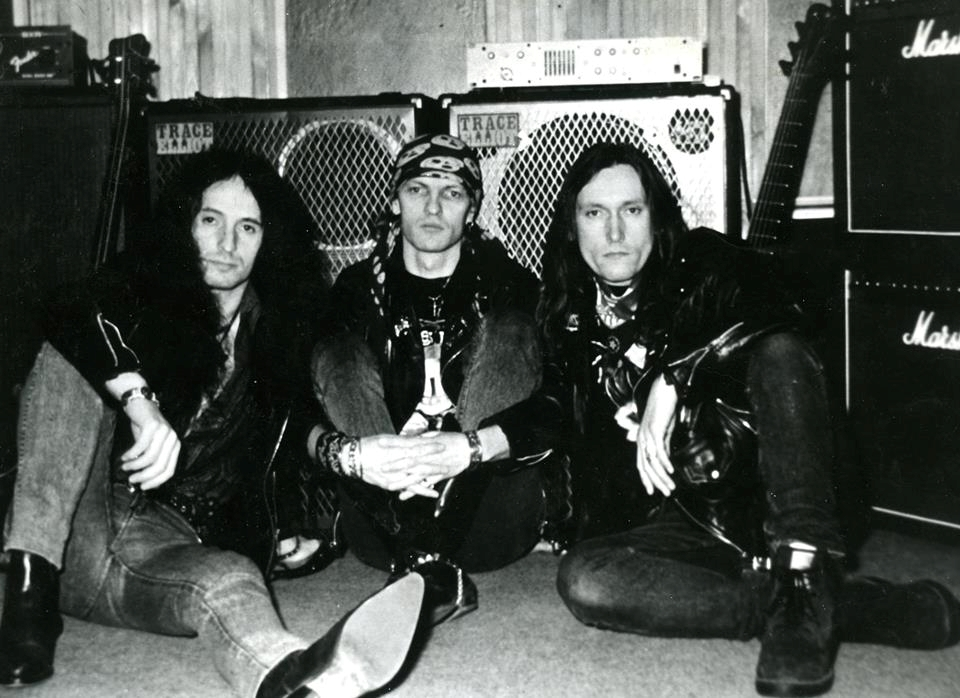
\includegraphics[scale=0.8]{Image27}
    \caption{\textit{Грановский, Большаков и Серышев на студии «SNC».}}
\end{figure}

Дождливый август 1991 года стал для «Мастера» полосой препятствий, которую преодолели немногие. Еще вчера могучая группа
развалилась на глазах. Несмотря на то, что пластинка была записана и Паскаль чуть ли не каждый день звонил в Москву с
вопросом, когда «Мастер» сможет выступать в Бельгии, «Мастер» не мог ехать на гастроли, так как у группы просто не было
работоспособного состава.

Альбом «Talk of The Devil» записывали барабанщики Сергей Ефимов («Круиз»), Владимир Ермаков («Черный Обелиск»), Андрей
Моисеев («Тяжелый День»), а также приятель Большакова по «Зигзагу» Павел Чиняков. В поездках, которые случились в то
время — в Кишинев и на фестиваль «Монстры рока» — с «Мастером» работал Андрей Шатуновский. Лишь потом в группе
«Мост-Дельта», игравшей на разогреве у «Арии», Большаков разглядел Анатолия Шендера, ставшего штатным барабанщиком
«Мастера».

\begin{figure}
    \centering
    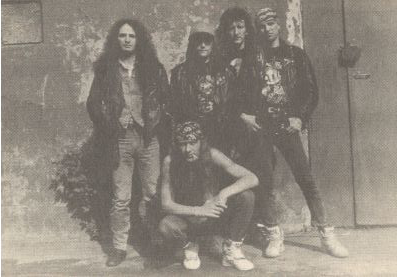
\includegraphics[scale=0.8]{Image28}
    \caption{\textit{«Мастер»-91: Грановский, Серышев, Кожин, Большаков, сидит Шендер}}
\end{figure}

А вот найти подходящего гитариста оказалось намного сложнее. Некоторое время с группой играл Игорь Кожин, но он был
блюзовым гитаристом, что не совсем сочеталось со стилем «хэви-металл». Затем место Кожина занял гитарист Вячеслав
Сидоров из группы «Хеллер», найденный вездесущим Большаковым. Сидоров вполне подходил «Мастеру», но после того как в
январе 1992 года правительство отпустило цены, концертная и тем более гастрольная жизнь страны замерла. У артистов не
было денег на дорогу к месту гастролей, а у зрителей не было денег, чтобы купить билеты на концерт. Поэтому «Мастер»
сыграл с Сидоровым лишь два концерта, и то в Москве — в только что открывшихся клубах «Секстон» и «Вояж».

\begin{figure}
    \centering
    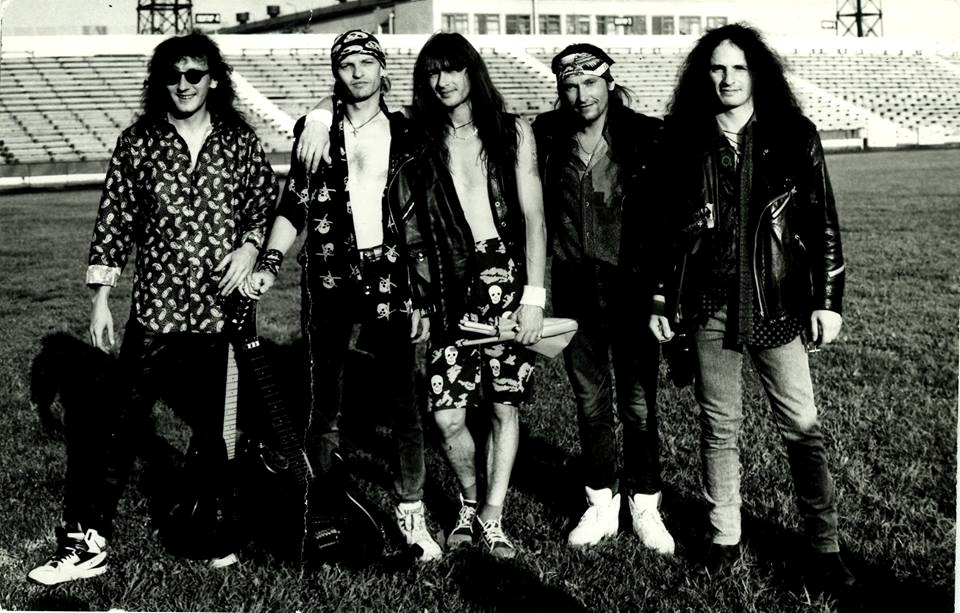
\includegraphics[scale=0.8]{Image29}
    \caption{\textit{«Мастер» в Павлодаре (1991 г.): Кожин, Большаков, Шендер, Серышев и Грановский}}
\end{figure}

Можно было вернуться в Бельгию, для «Мастера» это был бы лучший выход. Не каждая отечественная рок-группа имела
возможность укрыться от Гайдаровской шоковой терапии за границей, и музыканты, в принципе, собирались это сделать, но
тут тяжело заболел Андрей Большаков. Пришлось отменять запланированную поездку в Бельгию, поскольку заменить Большакова
в тот момент было просто невозможно. А сам Андрей не мог заниматься даже административной работой. «Знаешь, Алик, —
сказал он Грановскому, — теперь делай все сам. Если хочешь, устраивай концерты\ldots».

Ожидая выздоровления друга и чтобы как-то скоротать время, Грановский сочинял новые песни в актуальном тогда стиле
«прогрессив-трэш». Тексты вновь были английскими, так перед группой стояла цель вернуться в Бельгию с новым материалом.
В конце зимы 1993 года Грановский договорился со студией Центра Стаса Намина записать альбом, который позже получил
название «Мaniac Party». Большаков иногда приходил на студию, смотрел, что делают его друзья, слушал новый материал и
однажды даже попробовал что-то записать. Но работать в полную силу Андрей уже не мог, поэтому на альбоме остались лишь
несколько сыгранных им нот — они сохранились в песне «Screams of Pain»\ldots А тут еще в самый разгар записи Сидоров
разругался с Грановским и Серышевым и объявил, что уходит из «Мастера»\ldots

Еще осенью Грановский по пути на репетицию встретил на бульваре жену Сергея Попова. Она сразу же радостно защебетала:
«Алик, ну куда же вы все пропали?! Сергей постоянно о вас вспоминает\ldots Он так хочет играть!.. Алик, ну ты хоть
позвонил бы ему как-нибудь!.. Как у вас дела-то?!». «Идут дела потихоньку\ldots» — ответил Алик, хотя, если говорить
честно, дела никак и никуда не двигались вовсе.

И вот когда Сидоров отправился искать лучшую долю, Грановский позвонил Попову: «Сережа, ты не мог бы прийти на студию и
соло сыграть?». Попов пришел и сыграл все оставшиеся соло на альбоме «Maniac Party», без проблем уложившись в полсмены.

Почти сразу же после записи этого альбома у «Мастера» планировалась поездка на Украину. Грановский, Серышев и Крустер
сидели на базе и размышляли, как им быть? Большаков был близким другом, но в данный момент был болен и уже не мог
играть. В отличие от Андрея Попов был «готов к труду и обороне», к тому же он знал все партии, ему не требовалось учить
репертуар. Примерно в это время Андрей Большаков сообщил своим друзьям, что больше не может и не хочет заниматься
музыкой, и Попов фактически сразу получил предложение войти в состав группы, от которого он не стал отказываться.

Итак, «Мастер» в составе: Михаил Серышев (вокал), Алик Грановский (бас), Сергей Попов (гитара) и Анатолий Шендер
(барабаны) отправился в гастроли на Украину, затем — в Ростов-на-Дону и Краснодар. Вообще, для того смутного времени у
«Мастера» было довольно много концертов, хотя это был уже совсем не тот оглушительный успех, что сопровождал группу в
конце 80-х. Переход к бескомпромиссному «трэшу» значительно сузил потенциальную аудиторию группы, в результате
выступления переместились из Дворцов спорта в клубные залы. В Бельгии трэшевая программа шла «на ура», но когда «Мастер»
с этой же музыкой стал выступать в России, то группа сразу же растеряла большинство своих старых поклонников. Наша
публика предпочитает музыку мелодичную, а в «трэше» мелодичности мало, зато с избытком присутствует эмоциональное
напряжение, тяжелое для восприятия\ldots

Возможно, если бы у «Мастера» не было возможности параллельно работать Бельгии и группа выступала только на родине,
альбомы «Talk of The Devil», и «Maniac Party» вышли бы на русском языке. Но как только работа над «Maniac Party» была
завершена, Грановский созвонился со своими бельгийскими друзьями и сказал им, что пора «заряжать» концерты.

И тут возникли неожиданные проблемы с Серышевым. За период бездеятельности, что возник в связи с полураспадом группы в
1991 году, каждый искал, чем бы ему заняться и как заработать денег. Если Грановский, Попов и Шендер иногда записывались
как сессионные музыканты, то Серышев устроился петь в хор святой обители Михаила Архангела. Потом Михаил был приглашен в
академический хор, музыка которого оказалась весьма востребована. Хор стал много ездить по заграничным гастролям,
Серышев с новыми товарищами часто уезжал в поездки на месяц, а то и на два. И очень часто получалось так, что «Мастеру»
предлагали сыграть концерт, а Серышева в этот момент в Москве не было — от концертов приходилось отказываться. Про
«Мастер» даже стали поговаривать: «Ах, «Мастер»? А чего их приглашать, если у них нет состава?». Если в начале своей
истории «Мастер» работал как хорошо отлаженный механизм, то теперь он частенько просто не был готов к работе\ldots

\ldotsТак прошли три года. Страна потихонечку стала оправляться от кризиса, в начале 1995 года ожил и «Мастер». Первым
делом, чтобы напомнить поклонникам о себе, группа выпустила концертный альбом. Это была запись, сделанная во время
выступления в Таганском парке, где «Мастер» исполнил песни с альбомов «Talk of The Devil» и «Maniac Party», кстати, еще
нигде не изданных, а также несколько своих старых испытанных хитов — «Воля и Разум», «Палачи», «Здесь куют металл».

А потом наши герои нашли в себе силы и записали альбом на русском языке — «Песни мертвых». Полностью этот альбом имеет
название «Песни мертвых для живых», но на самом деле это — праздничная песнь живых, преодолевших испытания начала 90-х.
При этом живые склоняют головы перед теми, кто пал за рок-н-ролл. Поэтесса Маргарита Пушкина почувствовала это
настроение в новой музыке «Мастера» и посвятила заглавную песню альбома умершему в 1994 году Курту Кобейну. Что касается
музыки, то на этом альбоме «Мастер» вернулся к своему раннему мелодичному стилю, в результате чего «Песни мертвых» имели
успех, а баллада «Пепел на ветру», даже стала одним из ярких хитов 1996 года\ldots

Летом 1997 года «Мастер» все ж таки вырвался на концерты за рубеж, во Францию. Так как Серышев был как всегда плотно
занят в своем хоре, то Грановский принялся лихорадочно оглядываться по сторонам в поисках замены и вдруг обнаружил на
обочине шоу-бизнеса Артура Беркута, после продолжительного отсутствия вернувшегося в Москву из Соединенных Штатов. Одним
жарким июльским утром Грановский позвонил Беркуту:

— Артур, у нас жуткая проблема!
— Что случилось?
— Артур, только не говори «нет»! Через пять дней мы вылетаем во Францию, а Серышев отказался ехать. А мы должны ехать и
очень подведем человека, который нас пригласил.
— Алик, ты с ума сошел! «Мастер» и я – это совершенно разные вещи.
— Я знаю: ты сможешь.
— Но у меня даже загранпаспорта нет, у меня только американский паспорт, по которому меня выпустят только в Штаты.
— Мы сделаем тебе паспорт! И визу сделаем! Только не говори «нет»!

\begin{figure}
    \centering
    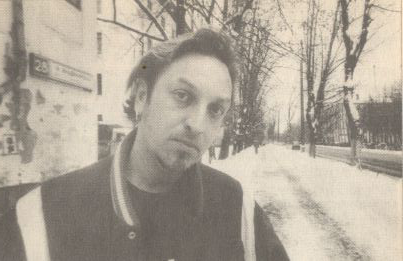
\includegraphics[scale=0.8]{Image30}
    \caption{\textit{Артур Беркут после возвращения из Франции}}
\end{figure}

Как и «Мастер», группа Артура Беркута «Автограф» в 1989 году уехала за границу, только не в Европу, а сразу — в США,
подписав контракт на запись альбома с фирмой «Capitol Records». В то время уезжали многие — «Аквариум» и «Круиз», «Шах»
и «Парк Горького», «арийцы» Маврин с Дубининым и «Ва-банкъ», — это было массовое поветрие, но за рубежом судьба у
большинства сложилась неудачно. «Автограф» попал в число неудачников. Группа записала в Америке пластинку (она
называлась «Turm Down The Border»), которой сами музыканты остались крайне недовольны, посколько продюсеры фирмы
«Capitol» упростили извилистые арт-роковые аранжировки «Автографа», доведя музыку группы до модных в то время в Америке
прямолинейных истин. В итоге успеха эта пластика не имела, часть музыкантов вернулись на родину, даже не отыграв до
конца промоушн-тур. А Беркут женился на американке и остался в Лос-Анджелесе. В 1993 году он попробовал вместе с
Леонидом Гуткиным, басистом «Автографа», еще раз завоевать Америку — и снова безрезультатно: целый год непрерывных
усилий не дал положительных результатов. Однако Артур не желал сдаваться. В музыкальной газете он прочитал объявление о
том, что группа с экзотическим для тех мест названием «Sibiria», исполняющая музыку в стиле «глэм», ищет вокалиста.
Артур приехал к ним на базу, спел пару песен и был принят в состав. В 1996 году группу услышал известный на западном
побережье продюсер Дэнис Маккэй (Dennis McCay), известный работой с Фрэнком Заппой (Frank Zappa), он предложил сменить
стиль на более современный «грандж», а заодно поменять и название. Так родилась группа «Zooom», получившая название по
имени известного лос-анджелесского порно-клуба, где собирались рокеры – его как раз тогда закрыли. «Zooom» вскоре стал
довольно популярным клубным коллективом на Западном побережье, у него вышел альбом, основную массу песен для которого
сочинил Беркут.

В это время из России стали доноситься звуки нового рок-карнавала, и звездам, уехавшим за границу, захотелось принять в
нем участие. В 1996 году многие музыканты стали возвращаться домой, но они опоздали. Уже сложилось новое рок-сообщество,
появились другие герои, зазвучали иные песни. Беркут изо всех сил старался быть актуальным, даже вызвал из Лос-Анджелеса
музыкантов своей американской группы. Однако дела шли неважно, выступлений почти не было. Так что предложение «Мастера»
подоспело как нельзя кстати\ldots

На репетиции оставалось пять дней, за это время Беркут должен был разучить песни «Мастера». «Да эти Ритины тексты
невозможно запомнить!» — жаловался Артур. И первый концерт во Франции он пел, весь обложенный листочками с текстами
песен. Но потом все вошло в свою колею: постоянные аншлаги, масса визжащего и трясущего волосами народа, летающие
лифчики экзальтированных поклонниц. Практически в каждом городе музыкантов приглашали в радиоэфир: «А вот – русская
группа! — привычно восторженно кричал в микрофон ди-джей — Она называется «Мастер». Эти люди сейчас у нас в студии.
Звоните, задавайте свои вопросы, они обо всем вам сейчас расскажут!..»

Два месяца «Мастер» колесил по городам Франции, но, к сожалению, все хорошее когда-нибудь кончается. Поздней осенью
группа вернулась в Москву, в слякоть и сырость, туда, где песни группы отсутствовали в ротации радиостанций и
хит-парадах. В довершение всего и Серышева не оказалось в Москве, он тоже поехал за рубеж, где его хор записывался с
Мэннфредом Мэнном (Manfred Mann). (Рассказывают, что английский музыкант сказал, указывая на Серышева: «На рокера похож»
— «А он и есть рокер!» — ответили коллеги Михаила.)

Грановский снова позвонил Беркуту, спросил, что Беркут собирается делать дальше и предложил сыграть концерт.

— Мы же вроде на одну поездку договаривались? — удивился Артур.
— Конечно! Но ты же понимаешь, что наши фэны хотят услышать, как мы звучали во Франции, — нашел предлог Грановский.
— Хорошо! Давай! — согласился Беркут.

Но зимой 1997 — 1998 годов «хэви-металл» в Москве был почти никому не нужен. Клубы требовали чего-нибудь
альтернативного, в крайнем случае соглашались на модные в то время анплагдовые (от англ. unplugged – неподключенный)
выступления. И тогда Сергей Попов предложил Беркуту сделать русский вариант «Zooom». Он рассчитывал, что с музыкой
«средней тяжести» можно будет выступать по клубам, которых к тому времени в Москве открылось уже довольно много. Попов и
Беркут начали репетировать программу «Zooom» на базе «Мастера». Когда об этом узнал Грановский, он страшно рассердился.

\begin{wrapfigure}{L}{0.5\textwidth}
    \centering
    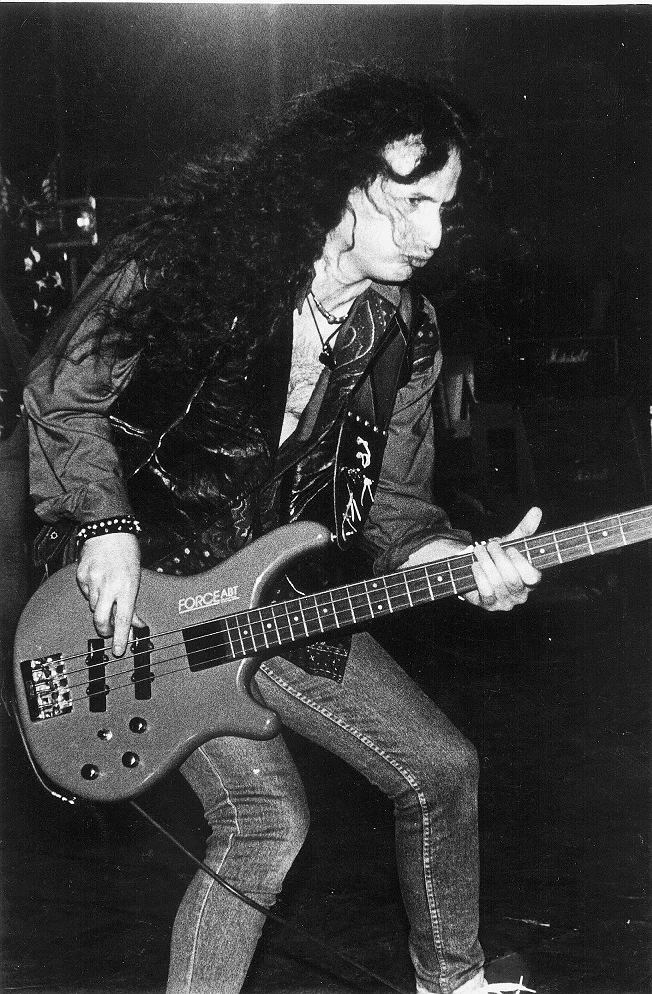
\includegraphics[scale=0.9]{Image31}
    \caption{\textit{Алик Грановский}}
\end{wrapfigure}

\begin{wrapfigure}{R}{0.5\textwidth}
    \centering
    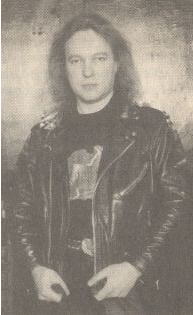
\includegraphics[scale=0.9]{Image32}
    \caption{\textit{Андрей Крустер-Лебедев}}
\end{wrapfigure}

— Ах так! — в ответ возмутился Попов, — тогда мы вообще сваливаем, потому что нам «Zooоm» играть интереснее!

Позицию Попова и Беркута поддержал и Шендер. Они решили: «Нам легче найти нового бас-гитариста и играть эту
музыку\ldots».

Грановского поддержали лишь Андрей Крустер и администратор группы Александр Лодыченко, в итоге новый 1998 год «Мастер»
встретил в новом составе. В группу вместо ушедших были приглашены гитарист Леонид Фомин (экс-«Валькирия) и барабанщик
Олег Милованов (экс-«Паранойя», «End Zone»). Милованов был близким приятелем Шендера и потому был в курсе всего, что
происходило в «Мастере». Когда Попов с Шендером ушли из группы, он позвонил Грановскому и сказал, что сейчас
свободен\ldots В свою очередь Милованов позвал в группу своего приятеля Леонида Фомина. Перед прослушиванием Фомин взял
домой кассету с песнями «Мастера», выучил пару гитарных партий, сыграл их и был принят в группу.

Оставалось найти солиста. «У меня был выбор между двумя решениями, — рассказывает Грановский, — или набрать абсолютно
новых музыкантов, взяв новое название, или пригласить Серышева, голос которого на протяжении многих лет был визитной
карточкой «Мастера», и сохранить название. Я не нашел ни одной причины, почему я должен избавиться от названия «Мастер»,
ведь я отдал этой группе двенадцать лет своей жизни\ldots». Решившись на подобный шаг, Грановский набрал номер Серышева:

— Миша, давай обратно!
— Давай! — просто ответил тот\ldots

Как только Серышев вернулся в состав, у «Мастера» все наладилось с концертной деятельностью. Удивительно, но именно это
стало причиной нового кризиса, ведь Серышев, кроме сотрудничества с двумя хорами, получил приглашение из театра
«Геликон-опера», где начал репетировать роль Звездочета в опере «Золотой петушок». Если бы «Мастер» по-прежнему вел
вялотекущую концертную жизнь, то Михаил успевал бы везде, но группа вновь стала получать множество приглашений на
концерты и гастроли, поэтому часто на сообщения Грановского о концертах «Мастера», Серышев отвечал: «Извини, я не
могу\ldots Я в этот день занят\ldots».

Но вот наступил 1999 год. Многие рокеры стали разучивать народные песни, некоторые поменяли гитары на сказочные духовые
инструменты, а для Грановского возвращение к корням означало капитальный ремонт «Мастера»: он решил расстаться с
Серышевым. Он долго колебался, прежде чем пойти на этот шаг, но ему пришлось сделать это, ведь не могут же трое взрослых
людей все время ждать одного?! Серышев спокойно принял это решение, поскольку давно уже пребывал в другом амплуа, и
разрываться между рок-музыкой и классикой уже не хотел.

Узнав, что в «Мастере» вакантно место вокалиста, на репетиционную базу группы в Кунцево потянулись певцы, иные с очень
похожими на Мишин голосами. Один из соискателей как и Серышев пел в церковном хоре. Он пообещал: «Если вы меня возьмете,
я уйду из храма!». «Не надо ниоткуда уходить!» — ответил Алик и отказал претенденту.

Грановский хорошо понимал, что заменой музыканта, на протяжении десяти лет являвшегося культовой фигурой российской
металлической сцены, не мог быть его голосовой двойник. Алик решился кардинально изменить стилистику группы. Поиски
продолжались до октября 1999 года. Как-то раз Грановский разговаривал с гитаристом «Арии» Сергеем Терентьевым и тот,
зная о проблеме «Мастера» с вокалистами, посоветовал прослушать Лекса, певца группы «Life», репетировавшего на базе
«Арии». Терентьев с таким восторгом рассказывал про этого парня, что заинтриговал Грановского. На следующий день Алик
позвонил Лексу. Их первый разговор получился весьма немногословным.

— Ты сразу не отказывайся, — сказал Алик, — ты подумай\ldots
— Почему нет? — ответил Лекс. — Давай попробуем.

На следующий день они встретились на базе у «Мастера», поиграли вместе старый добрыЙ «Deep Purple», и вопрос с
вокалистом был решен.

Широкой публике «Мастер» представил своего нового певца в январе 2000 года на концерте во Владимире. Следом была поездка
в Питер. Алику хотелось в полной мере удостовериться в том, что Лекс — тот человек, который достоин и сможет работать в
«Мастере». И только феврале на торжествах по случаю открытия «Р-клуба» Лекс появился перед столичными поклонниками
«Мастера». Причем даже афишах было заявлено не выступление группы «Мастер», а «музыкантов из группы «Мастер», которые
подготовили кавер-версии старых «фирменных» хитов. И только после этого выступления в «P-клубе» Лекс был официально
принят в группу.

Вновь началась череда концертов и гастролей. Снова замелькали за окнами поездов и автобусов пейзажи с полями, лесами,
реками и убегающими километровыми столбиками. Залы как прежде стали взрываться овациями. Для Лекса это стало вторым
рождением, оказалось, что приглашение от Грановского он получил в момент, когда уже решил завязать с музыкой. «В группе
«Life» мы работали с хорошими песнями, но все они когда-то и кем-то уже были сделаны, а тут — творчество, которое идет
от тебя, от людей, которые рядом с тобой, и когда ты чувствуешь эту связь, эти зацепки друг с другом, это, наверное,
лучшее, что есть в жизни! Да, пришлось работать с большей самоотдачей. Но как еще можно работать?! Если не так, то лучше
вообще не работать. А тем более такие песни, такие эмоции, если они откровенны, если они честны, по-другому передать
невозможно\ldots — говорил Лекс. — Эта музыка меня оживила, дала то, что я в этой жизни уже начал забывать\ldots» В
«Мастере» Лекс вновь обрел вкус к рок-музыке, а это — волшебное чувство.

\begin{figure}
    \centering
    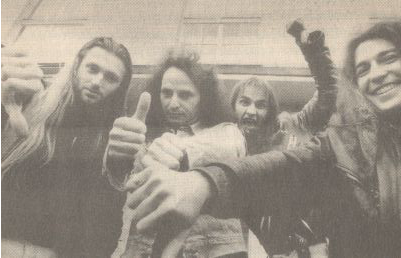
\includegraphics[scale=0.6]{Image33}
    \caption{\textit{«Мастер» - 1999: Фомин, Грановский, Милованов, Лекс.}}
\end{figure}

С приходом Лекса у «Мастера» словно выросли крылья, и группа начала работу над новым альбомом, получившим название
«Лабиринт».

Этот альбом в иносказательной форме рассказывает о приключениях «Мастера» в лабиринте ХХ века. Недаром в качестве
бонус-трека на нем записана песня «Таран» из репертуара ныне легендарной группы «Смещение», в которой Грановский играл в
начале своего музыкального пути. Но биография группы «Мастер» — это и биография целого поколения, пережившего
«високосный век» и вступившего в век XXI-й, с которым связаны чаяния и надежды, не сбывшиеся в веке минувшем.

Однако приключения «Мастера» не закончились. С наступлением 2001 года группа «Валькирия» возобновила свои выступления, и
гитарист Леонид Фомин вернулся в свой старый коллектив. И снова на выручку «Мастеру» пришел «ариец» Терентьев. Он
посоветовал Грановскому обратить внимание на виртуозного гитариста Страйка, к тому же являвшегося страстным поклонником
группы «Мастер» и знавшего репертуар группы. Страйк пришел на прослушивание, сыграл песни «Берегись», «Воля и разум», и
Грановскому ничего не оставалось делать, кроме как заявить его в основной состав, тем более что буквально через пять
дней должен был состояться концерт «Мастера» на фестивале «Крустер-2001». Они репетировали каждый день и сумели
подготовить для этого фестиваля небольшую программу. А еще через несколько недель уже состоялся сольный концерт
«Мастера».

\begin{figure}
    \centering
    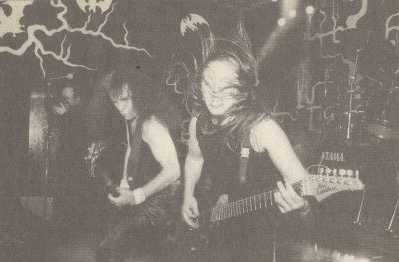
\includegraphics[scale=0.9]{Image34}
    \caption{\textit{«Мастер» в 2001 году: Алик Грановский и Страйк}}
\end{figure}

С появлением Страйка в «Мастере» возродился старый дух этой легендарной группы. В традиции «Мастера» устраивать кавардак
на сцене, Грановский с Большаковым всегда носились по сцене как сумасшедшие. Фомин категорически не хотел этого делать,
зато из Страйка энергия исходила таким мощным потоком, что позволяла устраивать на сцене настоящий цирк.

Кроме того, высокий профессиональный уровень Страйка позволил Грановскому реализовать давнюю мечту — сделать анплагдовую
программу. «Тяжелые» песни в акустическом варианте — это очень неожиданно и терпко\ldots

\begin{figure}
    \centering
    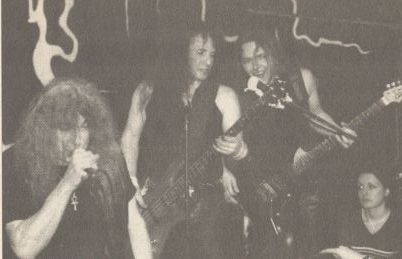
\includegraphics[scale=0.9]{Image35}
    \caption{\textit{Лекс, Грановский и Страйк}}
\end{figure}

В начале 2002 года срочно потребовалась замена барабанщику Олегу Милованову. Когда об этом разнесся по Москве слух,
барабанщики один за другим стали беспокоить Грановского. Одним из тех, кто позвонил в неурочный час, был Саша Карпухин
из группы Сергея Маврина. Он сказал, что хотел бы играть в «Мастере», но одновременно будет совмещать это с игрой у
Маврина. Грановский ответил, что с удовольствием взял бы его, но ему не хочется подставлять Маврина. На этом их общение
могло бы быть исчерпанным, но мама 17-летнего паренька позвонила Сергею Маврину и попробовала уговорить его разрешить
сыну параллельно играть в «Мастере». Сергей был категорически против подобного совмещения, так как он записывал новый
альбом, а кроме того на горизонте маячили гастроли его собственной группы. После этого разговора Саша позвонил
Грановскому и сказал, что будет играть только у Маврина. Но еще через три дня он перезвонил и сообщил, что принял
решение играть в «Мастере», потому что с детства является фанатом именно этой группы. Вот так юный музыкант стал
хозяином собственной реальности!..

30 апреля 2002 года «Мастер» большим концертом в ДК МАИ отмечал свое 15-летие. На юбилей явились все — Большаков,
Серышев, Шендер, Елин, а также несколько тысяч фанов. Сначала нынешний состав «Мастера» исполнил свою новую программу, а
потом на сцену вышли те, чьи имена принадлежат истории\ldots Большаков воткнул джек в комбик, дотронулся до струн, и они
запели в ожидании. Шендер пощекотал палочкой тугое брюхо барабана, и тот в ответ важно заурчал; микрофон приник своим
единственным, но чутким ухом к губам Серышева. Тут Грановский ударил по струнам, будто подал команду: «Пли!». И
загремели старые хиты — «Палачи», «Воля и Разум», «Встань, страх преодолей»\ldots

\begin{figure}
    \centering
    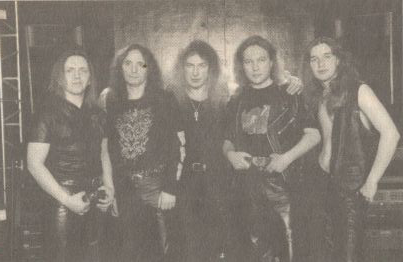
\includegraphics[scale=0.9]{Image36}
    \caption{\textit{«Мастер» в 2003 году}}
\end{figure}

«У меня там гитару заклинило, прямо на первой вещи, — вспоминает Андрей Большаков о том юбилейном концерте. — Мы
начинаем играть, а у меня выскочил винт пружины, который держит звукосниматель, и прилип к струнам. Я играю, а из гитары
идет звук, как у ситара: з-з-з-з\ldots Но ничего! Народ не очень понял, что происходит\ldots Перед этим концертом у нас
прошло три или четыре репетиции. Ребята вставили синкопы, изменили некоторые ходы, отдельные новые фрагменты появились,
например тема «Пер Гюнта», и это меня ужасно доставало, потому что все это нужно было учить. Тогда я предложил Алику:
«Давай, я не буду это разучивать! Я просто хочу сыграть ту музыку, которую сам написал когда-то вместе с тобой. Ты мне
мил-дорог, давай будем играть именно так, как делали это раньше! Зачем мне современные-то аранжировки учить?»

Эти вещи я не играл десять лет, я вообще все это время не играл на гитаре, и пальцы перестали меня слушаться. Но вот что
удивительно — за одну репетицию я все вспомнил, вернее я даже не вспоминал: руки сами стали играть. Все-таки эти вещи
уже сидят в подсознанье, тем более что я их сам сочинил! А на концерте я опять испытал давно забытое ощущение: как мне
кайфово играть с Аликом! Он этого, конечно, не знает, но мне с ним на сцене всегда было комфортно, и хотелось играть. А
когда еще Толик сел за барабаны и Миша вышел, то стало вообще здорово!

После концерта Толик Шендер мне говорит: «Андрюха, давай играть! Сделаем команду, возьмем Грановского, и будем втроем
мочить! И все будет клево!..»

Возможно, юбилейный концерт также стал точкой отсчета для чего-то нового и необычного. Но об этом мы узнаем лишь спустя
несколько лет\ldots

\begin{figure}
    \centering
    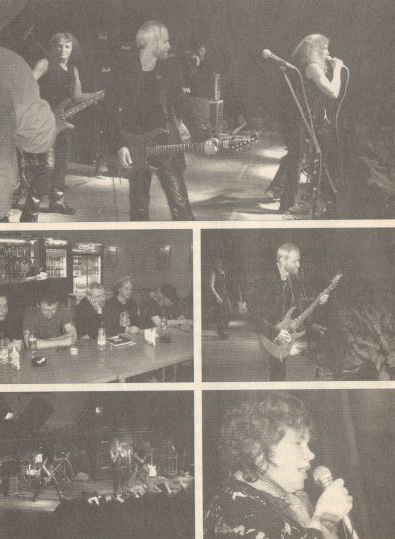
\includegraphics[scale=0.9]{Image37}
    \caption{\textit{Фотографии с юбилейного концерта «Мастера» в ДК МАИ}}
\end{figure}

\begin{figure}
    \centering
    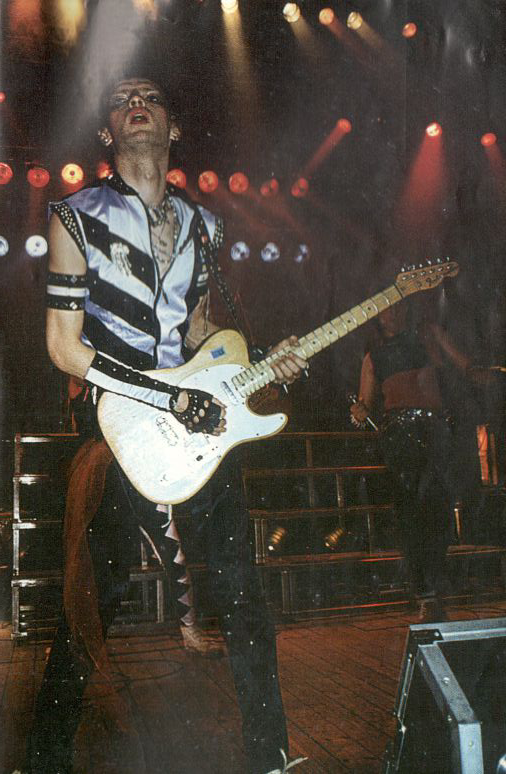
\includegraphics[scale=0.6]{Cover3}
\end{figure}

\begin{figure}
    \centering
    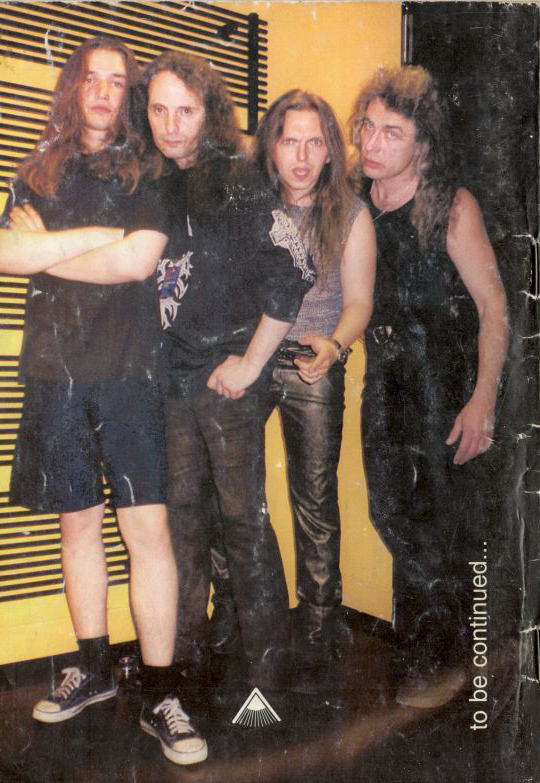
\includegraphics[scale=0.6]{Cover4}
\end{figure}

\end{document}
